\documentclass[a4paper,12pt]{report}

% ─── Packages ──────────────────────────────────────────────────────
\usepackage[utf8]{inputenc}
\usepackage[T1]{fontenc}
\usepackage[italian]{babel}
\usepackage{geometry}
\geometry{margin=2.5cm}
\usepackage{graphicx}
\usepackage{hyperref}
\hypersetup{
    colorlinks=true,
    linkcolor=blue!70!black,
    citecolor=blue!70!black,
    urlcolor=blue!60!black,
    pdfauthor={},
    pdftitle={Agentic UniBG – Relazione Finale},
}
\usepackage{enumitem}
\usepackage{tabularx}
\usepackage{booktabs}
\usepackage{longtable}
\usepackage{listings}
\usepackage{xcolor}
\usepackage{titlesec}
\usepackage{fancyhdr}
\usepackage{float}
\usepackage{caption}
\usepackage{microtype}
\usepackage{parskip}
\usepackage{amsmath}

% ─── Listings style ───────────────────────────────────────────────
\definecolor{codebg}{HTML}{F5F5F5}
\definecolor{codegreen}{HTML}{2E7D32}
\definecolor{codeblue}{HTML}{1565C0}
\definecolor{codegray}{HTML}{757575}
\definecolor{codepurple}{HTML}{7B1FA2}

\lstdefinestyle{codestyle}{
    backgroundcolor=\color{codebg},
    commentstyle=\color{codegreen}\itshape,
    keywordstyle=\color{codeblue}\bfseries,
    numberstyle=\tiny\color{codegray},
    stringstyle=\color{codepurple},
    basicstyle=\ttfamily\small,
    breakatwhitespace=false,
    breaklines=true,
    captionpos=b,
    keepspaces=true,
    numbers=left,
    numbersep=5pt,
    showspaces=false,
    showstringspaces=false,
    showtabs=false,
    tabsize=2,
    frame=single,
    rulecolor=\color{codegray!30},
}
\lstset{style=codestyle}

% ─── Headers / footers ────────────────────────────────────────────
\pagestyle{fancy}
\fancyhf{}
\fancyhead[L]{\small\leftmark}
\fancyhead[R]{\small Agentic UniBG}
\fancyfoot[C]{\thepage}
\renewcommand{\headrulewidth}{0.4pt}

% ─── Title formatting ─────────────────────────────────────────────
\titleformat{\chapter}[display]
  {\normalfont\huge\bfseries}{\chaptertitlename\ \thechapter}{18pt}{\Huge}
\titlespacing*{\chapter}{0pt}{-20pt}{30pt}

% ─── Graphics path ────────────────────────────────────────────────
\graphicspath{
  {../iterazioni/iterazione0/images/}
  {../iterazioni/iterazione1/images1/}
  {../iterazioni/iterazione2/images2/}
  {../iterazioni/iterazione3/images/}
  {../iterazioni/iterazione4/images4/}
}

% ═══════════════════════════════════════════════════════════════════
\begin{document}

% ─── Title page ────────────────────────────────────────────────────
\begin{titlepage}
\centering
\vspace*{2cm}

{\Huge\bfseries Agentic UniBG\par}
\vspace{0.5cm}
{\Large Sistema Multi-Agent per l'Assistenza Universitaria\par}
\vspace{1.5cm}
{\large Relazione Finale del Progetto\par}
\vspace{0.5cm}
{\large Metodologia AMDD -- Agile Model Driven Development\par}
\vspace{3cm}

{\large Università degli Studi di Bergamo\par}
\vspace{0.5cm}
{\large Anno Accademico 2025/2026\par}

\vfill
{\small Documento generato il \today\par}
\end{titlepage}

% ─── Table of contents ─────────────────────────────────────────────
\tableofcontents
\newpage

% ═══════════════════════════════════════════════════════════════════
% CHAPTER 1 – INTRODUZIONE
% ═══════════════════════════════════════════════════════════════════
\chapter{Introduzione}

\section{Contesto del Progetto}

Il sito web dell'Università degli Studi di Bergamo (\texttt{unibg.it}) presenta una struttura gerarchica complessa, con informazioni distribuite su numerose pagine e documenti. Studenti e utenti devono navigare manualmente tra molte sezioni o consultare documenti lunghi per ricercare una singola informazione, con conseguenti perdite di tempo.

\textbf{Agentic UniBG} nasce con l'obiettivo di sviluppare un sistema intelligente multi-agent in grado di assistere studenti e utenti nella navigazione del sito universitario, fornendo risposte rapide, contestualizzate e personalizzate a qualsiasi domanda pertinente.

\section{Obiettivi del Sistema}

Il sistema è concepito come un assistente conversazionale avanzato, capace di:
\begin{itemize}
    \item Comprendere richieste in linguaggio naturale
    \item Classificare automaticamente l'intento della domanda
    \item Recuperare informazioni reali e aggiornate dal sito dell'ateneo
    \item Generare risposte strutturate, accurate e contestualizzate
    \item Personalizzare l'esperienza in base al profilo dello studente
    \item Gestire conversazioni multi-turno con memoria del contesto
\end{itemize}

\section{Metodologia di Sviluppo: AMDD}

Il progetto adotta la metodologia \textbf{Agile Model Driven Development (AMDD)}, che combina i principi dello sviluppo agile con la modellazione iterativa e incrementale.

L'approccio AMDD prevede:
\begin{enumerate}
    \item \textbf{Iterazione 0 -- Envisioning}: definizione della visione iniziale, dei requisiti ad alto livello e dell'architettura target. Nessun codice prodotto.
    \item \textbf{Iterazioni successive}: sviluppo incrementale con cicli brevi, ciascuno dei quali produce un incremento funzionante del sistema. I modelli UML vengono creati e aggiornati ad ogni iterazione secondo necessità (``just enough modeling'').
    \item \textbf{Evoluzione continua}: i requisiti, l'architettura e la documentazione evolvono di pari passo con il codice, senza fasi rigide di design upfront.
\end{enumerate}

\section{Tecnologie Utilizzate}

\begin{table}[H]
\centering
\begin{tabularx}{\textwidth}{l X}
\toprule
\textbf{Componente} & \textbf{Tecnologia} \\
\midrule
Frontend & React (Vite), servito tramite Nginx \\
Backend & Python, FastAPI, Uvicorn \\
Framework AI & LangChain, LangGraph \\
LLM Provider & Google Gemini 2.5 Flash (precedentemente Groq / LLaMA 3.3 70B) \\
Ricerca Web & Tavily API (search + extract) \\
Gestione PDF & PyMuPDF (fitz) \\
Database & MongoDB Atlas (Motor async driver) \\
Autenticazione & JWT (python-jose), bcrypt, httpOnly cookie \\
Containerizzazione & Docker, Docker Compose \\
\bottomrule
\end{tabularx}
\caption{Stack tecnologico del progetto}
\end{table}

\section{Struttura del Documento}

Ogni capitolo relativo a un'iterazione segue una scaletta uniforme:
\begin{enumerate}
    \item \textbf{Obiettivo dell'iterazione}
    \item \textbf{Analisi dei requisiti e use case}
    \item \textbf{Design dell'architettura} (diagrammi di componenti, classi, sequenza, attività)
    \item \textbf{Testing dinamico} (test API con Postman)
    \item \textbf{Analisi statica del codice} (metriche con radon)
\end{enumerate}

Indice dei capitoli:
\begin{itemize}
    \item \textbf{Capitolo 2}: Iterazione 0 -- Visione iniziale
    \item \textbf{Capitolo 3}: Iterazione 1 -- MVP della pipeline multi-agent
    \item \textbf{Capitolo 4}: Iterazione 2 -- Autenticazione, profilazione e personalizzazione
    \item \textbf{Capitolo 5}: Iterazione 3 -- JWT, gestione sessione e memoria conversazionale
    \item \textbf{Capitolo 6}: Iterazione 4 -- Web search, date esami e pipeline logging
    \item \textbf{Capitolo 7}: Iterazione 5 -- Gestione profilo utente e miglioramenti (WIP)
    \item \textbf{Capitolo 8}: Scelte architetturali e di progetto
    \item \textbf{Capitolo 9}: Conclusioni e sviluppi futuri
\end{itemize}


% ═══════════════════════════════════════════════════════════════════
% CHAPTER 2 – ITERAZIONE 0
% ═══════════════════════════════════════════════════════════════════
\chapter{Iterazione 0 -- Visione Iniziale}

\section{Obiettivo dell'Iterazione}

L'Iterazione 0 rappresenta la fase di \textit{envisioning} prevista dalla metodologia AMDD. Non è stato prodotto codice funzionante, ma sono stati definiti:
\begin{itemize}
    \item La visione complessiva del progetto
    \item Le user stories iniziali (target completo)
    \item I requisiti funzionali e non funzionali ad alto livello
    \item L'architettura target del sistema
    \item I rischi iniziali identificati
\end{itemize}

\section{Analisi dei Requisiti e Use Case}

\subsection{User Stories Iniziali}

Le user stories della visione iniziale coprono l'intero spettro delle funzionalità desiderate:

\begin{table}[H]
\centering
\begin{tabularx}{\textwidth}{l X}
\toprule
\textbf{ID} & \textbf{Descrizione} \\
\midrule
US-01 & Come studente autenticato, voglio accedere al sistema con il mio profilo \\
US-02 & Come visitatore esterno, voglio porre domande senza autenticazione \\
US-03 & Come studente, voglio chiedere informazioni su un corso \\
US-04 & Come studente, voglio conoscere l'orario delle lezioni \\
US-05 & Come studente, voglio sapere se un'aula è libera \\
US-06 & Come studente, voglio trovare un regolamento o documento ufficiale \\
US-07 & Come studente, voglio essere guidato passo-passo in una procedura \\
US-08 & Come studente autenticato, voglio che il sistema ricordi le conversazioni \\
US-09 & Come utente, voglio fornire un feedback sulla risposta \\
\bottomrule
\end{tabularx}
\caption{User stories -- visione completa (Iterazione 0)}
\end{table}

\subsection{Use Case della Visione Completa}

Sono stati identificati 13 macro-casi d'uso, suddivisi per attore:

\begin{table}[H]
\centering
\small
\begin{tabularx}{\textwidth}{l l X}
\toprule
\textbf{ID} & \textbf{Attore} & \textbf{Nome} \\
\midrule
UC-01 & Studente & Login come Studente \\
UC-02 & Studente & Registrazione Studente \\
UC-03 & Studente & Gestione Profilo \\
UC-04 & Ospite & Accesso come Ospite \\
UC-05 & Studente, Ospite & Inviare Domanda/Richiesta \\
UC-06 & Studente & Richiedere Guida Procedurale \\
UC-07 & Studente & Recupero Documento Ufficiale \\
UC-08 & Studente & Informazioni su un Corso \\
UC-09 & Studente & Consultazione Orari Lezioni \\
UC-10 & Studente & Verifica Occupazione Aule \\
UC-11 & Studente, Ospite & Informazioni Generali \\
UC-12 & Studente, Ospite & Ricevere Risposta \\
UC-13 & Studente, Ospite & Fornire Feedback \\
\bottomrule
\end{tabularx}
\caption{Use case della visione completa (Iterazione 0)}
\end{table}

\begin{figure}[H]
\centering
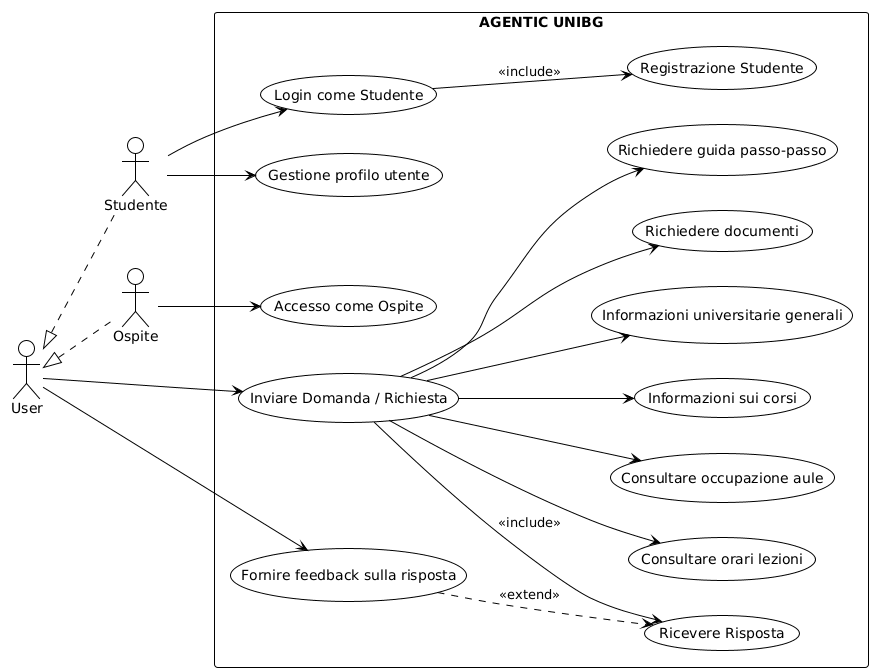
\includegraphics[width=0.85\textwidth]{usecase_diagram0}
\caption{Diagramma dei casi d'uso -- Iterazione 0}
\end{figure}

\subsection{Rischi Iniziali e Strategia}

\begin{itemize}
    \item \textbf{Complessità architetturale elevata}: mitigata dalla scomposizione in iterazioni incrementali
    \item \textbf{Dipendenza da servizi LLM esterni}: mitigata dalla modularità (sostituzione provider trasparente)
    \item \textbf{Incertezza sulla qualità delle risposte}: mitigata dall'introduzione del Revision Agent e delle fonti web
\end{itemize}

La strategia adottata prevede di procedere per \textit{minimum viable product} incrementali, evolvendo l'architettura progressivamente.

\section{Design dell'Architettura}

L'architettura target prevede tre macro-componenti:
\begin{enumerate}
    \item \textbf{Frontend}: applicazione React per l'interazione utente (login, chat)
    \item \textbf{Backend (LangChain)}: API Gateway, Orchestrator Agent e agenti specializzati (Classifier, Profile, Memory, Web, Documents, Generator, Revision, Feedback)
    \item \textbf{Persistence Layer}: database per profili studente e cronologia conversazioni
    \item \textbf{Componenti esterni}: LLM Provider, accesso web
\end{enumerate}

\subsection{Diagramma dei Componenti}

\begin{figure}[H]
\centering
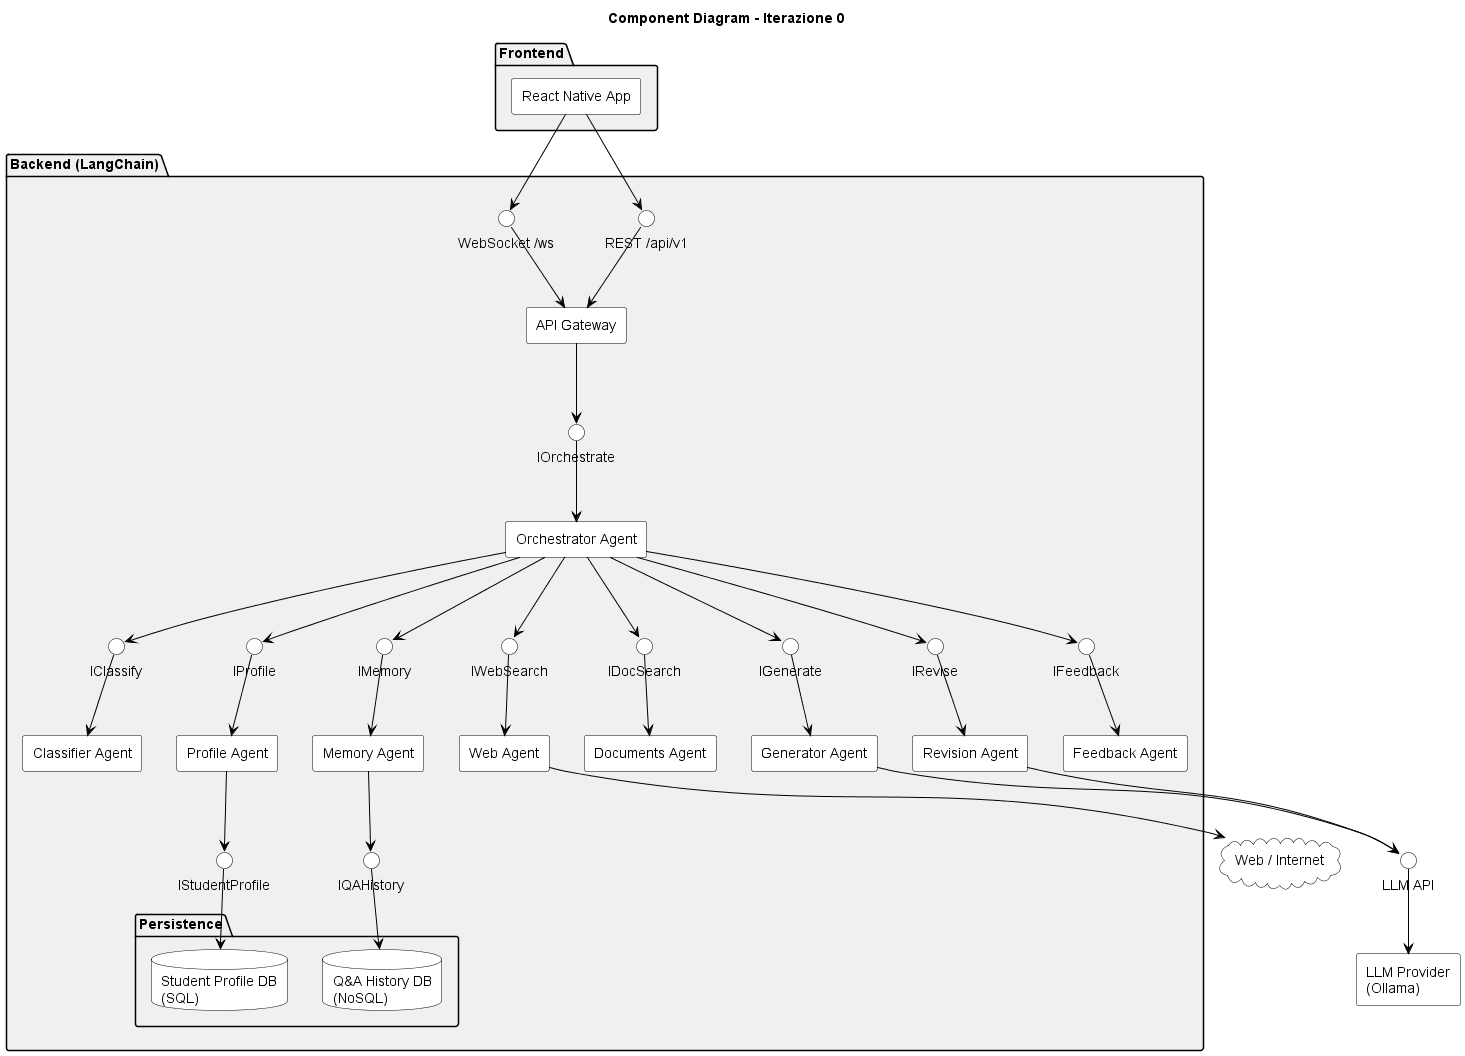
\includegraphics[width=\textwidth]{component_diagram0}
\caption{Diagramma dei componenti -- Architettura target (Iterazione 0)}
\end{figure}

\subsection{Diagramma degli Agenti}

\begin{figure}[H]
\centering
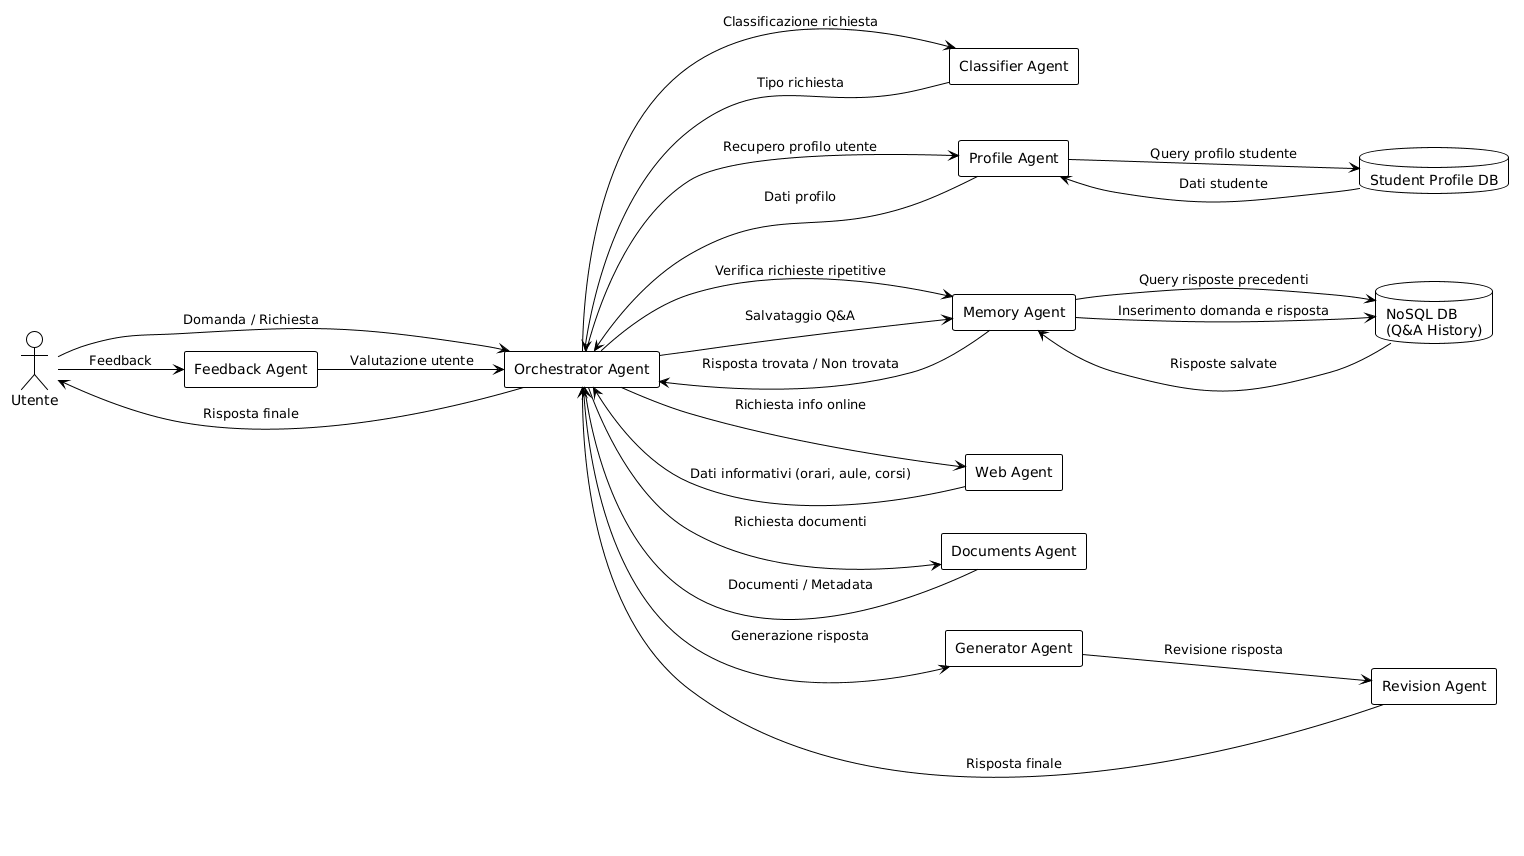
\includegraphics[width=0.9\textwidth]{agents__diagram0}
\caption{Diagramma degli agenti previsti -- Iterazione 0}
\end{figure}

\section{Testing Dinamico}

Non applicabile: l'Iterazione 0 è una fase di envisioning senza codice prodotto.

\section{Analisi Statica del Codice}

Non applicabile: nessun codice sorgente prodotto in questa iterazione.


% ═══════════════════════════════════════════════════════════════════
% CHAPTER 3 – ITERAZIONE 1
% ═══════════════════════════════════════════════════════════════════
\chapter{Iterazione 1 -- MVP della Pipeline Multi-Agent}

\section{Obiettivo dell'Iterazione}

Implementare il primo \textbf{Minimum Viable Product (MVP)} funzionante, limitato alla pipeline conversazionale di base: ricezione della domanda, classificazione dell'intento, generazione della risposta e revisione.

L'architettura è organizzata in \textbf{due tier} (Client + Application Logic), senza Data Tier, autenticazione o personalizzazione.

\section{Analisi dei Requisiti e Use Case}

\subsection{User Stories}

\begin{table}[H]
\centering
\begin{tabularx}{\textwidth}{l X}
\toprule
\textbf{ID} & \textbf{Descrizione} \\
\midrule
US-10 & Come studente, voglio inviare una domanda testuale e ricevere una risposta \\
US-11 & Come sistema, voglio classificare la richiesta per generare una risposta coerente \\
US-12 & Come sistema, voglio generare una risposta tramite LLM pertinente alla domanda \\
US-13 & Come sistema, voglio verificare la qualità della risposta per ridurre errori \\
\bottomrule
\end{tabularx}
\caption{User stories -- Iterazione 1}
\end{table}

\subsection{Use Case}

\begin{itemize}
    \item \textbf{UC-I1 -- Invio Richiesta}: l'utente invia una domanda via \texttt{POST /api/agent/query}. Se la query è vuota il frontend blocca l'invio; se il backend fallisce viene mostrato un errore generico.
    \item \textbf{UC-I2 -- Classificazione Intento}: il ClassifierAgent invia un prompt strutturato all'LLM con le categorie disponibili. Se la categoria restituita non è valida, fallback a \texttt{altro}.
    \item \textbf{UC-I3 -- Generazione Risposta}: il GeneratorAgent costruisce un prompt contestualizzato alla categoria e invoca l'LLM.
    \item \textbf{UC-I4 -- Revisione Risposta}: il RevisionAgent revisiona la bozza. In caso di errore, la bozza originale viene usata come fallback (graceful degradation).
\end{itemize}

\subsection{Requisiti Non Funzionali}

\begin{itemize}
    \item \textbf{RNF-I1}: tempo di risposta $\leq$ 10 secondi
    \item \textbf{RNF-I2}: modularità -- ogni agente è indipendente e sostituibile
    \item \textbf{RNF-I3}: robustezza -- fallimento del RevisionAgent non blocca la pipeline
    \item \textbf{RNF-I4}: statelessness -- nessuna persistenza tra richieste
    \item \textbf{RNF-I5}: estensibilità -- aggiunta di nuovi nodi senza modifiche alla logica esistente
    \item \textbf{RNF-I6}: documentazione API tramite Swagger UI (\texttt{/docs})
\end{itemize}

\begin{figure}[H]
\centering
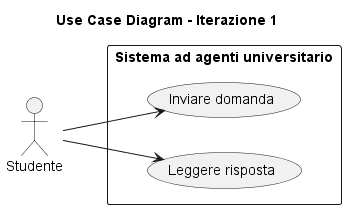
\includegraphics[width=0.8\textwidth]{usecase_diagram1}
\caption{Diagramma dei casi d'uso -- Iterazione 1}
\end{figure}

\section{Design dell'Architettura}

\subsection{Diagramma dei Componenti}

I componenti sviluppati sono:
\begin{itemize}
    \item \textbf{OrchestratorAgent}: costruisce il grafo LangGraph con tre nodi (\texttt{classify} $\rightarrow$ \texttt{generate} $\rightarrow$ \texttt{revise})
    \item \textbf{ClassifierAgent}: classifica la query in una delle 6 categorie
    \item \textbf{GeneratorAgent}: genera la risposta con prompt per categoria
    \item \textbf{RevisionAgent}: revisiona la bozza
    \item \textbf{AgentState}: \texttt{TypedDict} condiviso per lo stato della pipeline
\end{itemize}

\begin{figure}[H]
\centering

\includegraphics[width=\textwidth]{component_diagram1}
\caption{Diagramma dei componenti -- Iterazione 1}
\end{figure}

\subsection{Diagramma delle Classi}

\begin{figure}[H]
\centering
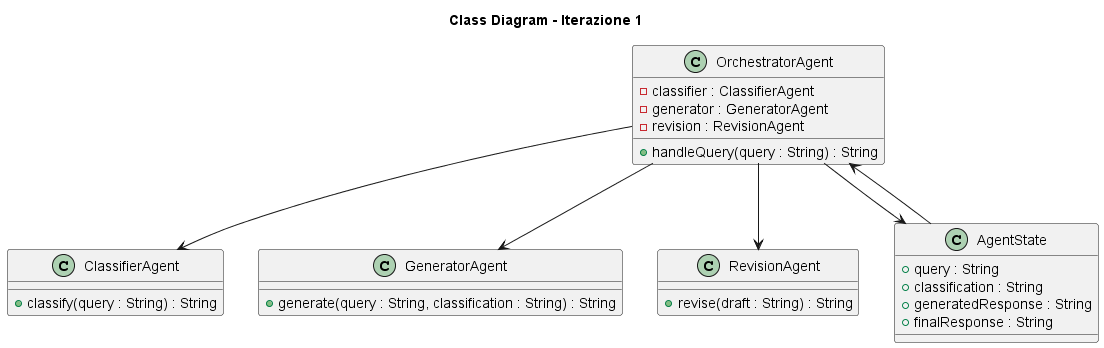
\includegraphics[width=\textwidth]{class_diagram1}
\caption{Diagramma delle classi -- Iterazione 1}
\end{figure}

L'\texttt{AgentState} contiene: \texttt{query}, \texttt{category}, \texttt{generated\_response}, \texttt{final\_response}, \texttt{workflow\_steps}, \texttt{status}.

\subsection{Diagramma di Sequenza}

\begin{figure}[H]
\centering
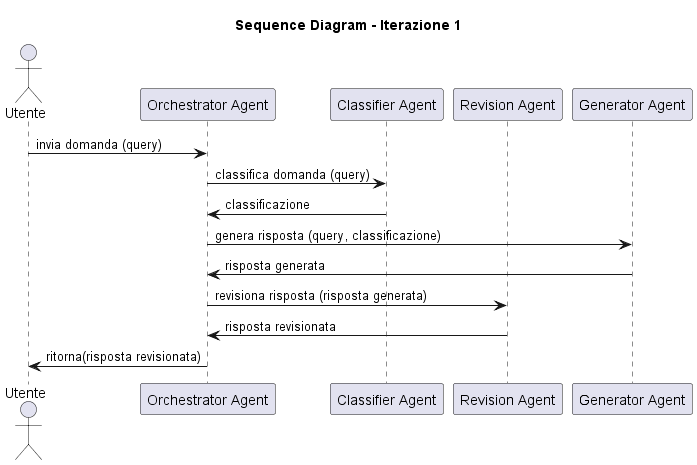
\includegraphics[width=\textwidth]{sequence_diagram1}
\caption{Diagramma di sequenza -- Pipeline classify $\rightarrow$ generate $\rightarrow$ revise}
\end{figure}

Il flusso sequenziale:
\begin{enumerate}
    \item L'utente invia la query all'OrchestratorAgent
    \item ClassifierAgent classifica l'intento
    \item GeneratorAgent genera la bozza
    \item RevisionAgent revisiona la risposta
    \item L'Orchestrator restituisce il risultato finale
\end{enumerate}

\subsection{Diagramma di Attività}

\begin{figure}[H]
\centering
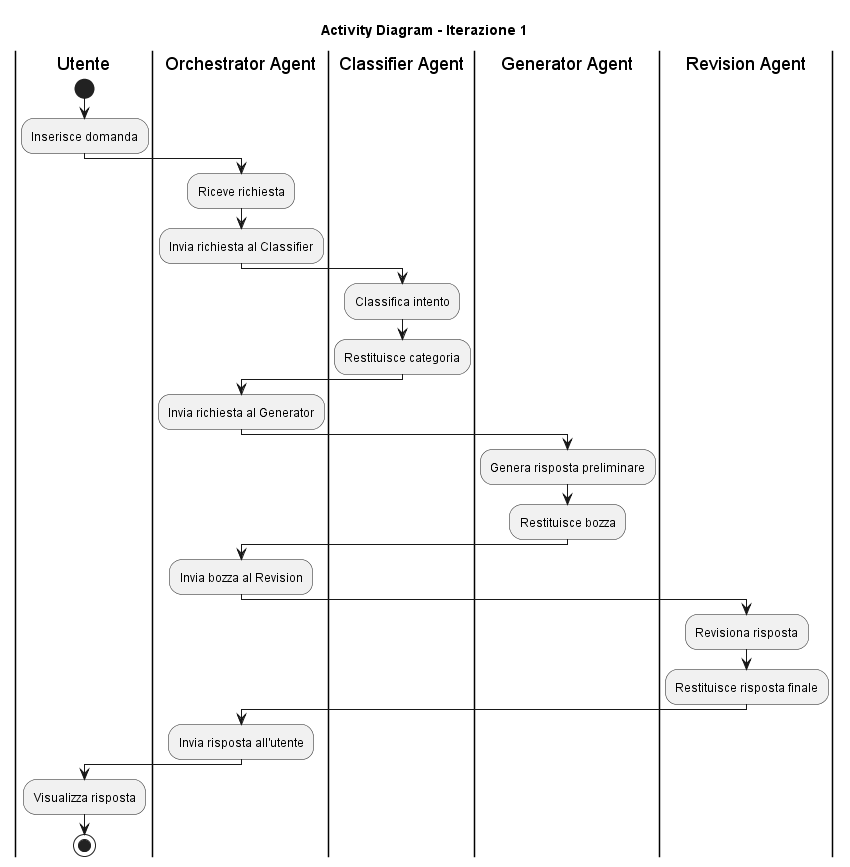
\includegraphics[width=0.75\textwidth]{activity_diagram1}
\caption{Diagramma di attività -- Pipeline Iterazione 1}
\end{figure}

\subsection{Algoritmi e Complessità}

\paragraph{Pipeline Orchestrator.}
Il workflow \texttt{classify} $\rightarrow$ \texttt{generate} $\rightarrow$ \texttt{revise} esegue 3 invocazioni LLM sequenziali. Complessità: $O(3L) = O(L)$, dove $L$ è il costo di una singola invocazione LLM (operazione I/O-bound dominante). Complessità spaziale: $O(n + R)$ dove $n$ è la lunghezza della query e $R$ la dimensione della risposta.

\paragraph{Classificazione.}
L'algoritmo di classificazione costruisce un prompt con $k=7$ categorie, invoca l'LLM, esegue parsing e validazione con fallback a \texttt{altro}. Complessità: $O(L)$, con lookup in dizionario $O(1)$ ammortizzato.

\section{Testing Dinamico}

I test API sono stati eseguiti con \textbf{Postman}. La collezione completa è in \texttt{postman\_collection.json}.

\begin{table}[H]
\centering
\small
\begin{tabularx}{\textwidth}{l l l X l}
\toprule
\textbf{ID} & \textbf{Endpoint} & \textbf{Metodo} & \textbf{Descrizione} & \textbf{Atteso} \\
\midrule
IT1-01 & \texttt{/api/health} & GET & Health check & 200 \\
IT1-02 & \texttt{/} & GET & Root endpoint & 200 \\
IT1-03 & \texttt{/api/agent/query} & POST & Query generica ospite & 200 \\
IT1-04 & \texttt{/api/agent/query} & POST & Query su docente & 200 \\
IT1-05 & \texttt{/api/agent/query} & POST & Query vuota & Errore \\
IT1-06 & \texttt{/api/agents} & GET & Lista agenti & 200 \\
\bottomrule
\end{tabularx}
\caption{Test API -- Iterazione 1 (6 test, 4 endpoint)}
\end{table}

\textbf{Variabili Postman}: \texttt{base\_url} = \texttt{http://localhost:8000}.

\textbf{Asserzioni chiave}: la risposta contiene sempre \texttt{response} (stringa non vuota), \texttt{agent\_used} e \texttt{metadata.workflow\_steps} con il tracking dei passi della pipeline.

\textbf{Esecuzione automatizzata}: tramite Newman CLI:
\begin{verbatim}
newman run postman_collection.json --folder "Iterazione 1"
\end{verbatim}

\section{Analisi Statica del Codice}

L'analisi statica è stata condotta con \textbf{radon} (Python). In questa iterazione sono presenti solo i moduli degli agenti e il server principale.

\textbf{Complessità ciclomatica}: tutti i moduli in grado \textbf{A} (CC $\leq$ 5), ad eccezione di \texttt{classify} (CC=6, grado B) per la logica di costruzione del contesto e validazione.

\textbf{Manutenibilità}: tutti i file in grado \textbf{A} (MI $>$ 20).

\textbf{Nota}: le metriche dettagliate per file sono riportate nella sezione di analisi statica cumulativa dell'Iterazione 4 (§\ref{sec:analisi-statica-completa}).


% ═══════════════════════════════════════════════════════════════════
% CHAPTER 4 – ITERAZIONE 2
% ═══════════════════════════════════════════════════════════════════
\chapter{Iterazione 2 -- Autenticazione, Profilazione e Personalizzazione}

\section{Obiettivo dell'Iterazione}

Evolvere il sistema verso un'applicazione completa e deployabile, introducendo:
\begin{itemize}
    \item Autenticazione utente (registrazione e login con matricola e password)
    \item Profilazione personalizzata (corso, dipartimento, anno, tipologia)
    \item Personalizzazione delle risposte tramite profilo utente
    \item Frontend React completo (SPA con login e chat)
    \item Persistenza su MongoDB Atlas (Motor async)
    \item Containerizzazione con Docker Compose
\end{itemize}

L'architettura evolve a \textbf{tre tier} (Client, Backend, Data). \textbf{Nota importante}: in questa iterazione il \textbf{JWT non è stato implementato}; il login restituisce direttamente il profilo senza token di sessione. La gestione JWT è stata rimandata all'Iterazione 3.

\section{Analisi dei Requisiti e Use Case}

\subsection{User Stories}

\begin{table}[H]
\centering
\begin{tabularx}{\textwidth}{l X l}
\toprule
\textbf{ID} & \textbf{Descrizione} & \textbf{Ruolo} \\
\midrule
US-01 & Registrazione con matricola e password & Studente \\
US-02 & Autenticazione e ricezione profilo & Studente \\
US-03 & Invio domande senza autenticazione & Ospite \\
US-04 & Risposte personalizzate in base a corso e anno & Studente \\
US-05 & Invio richiesta e ricezione risposta elaborata & Utente \\
\bottomrule
\end{tabularx}
\caption{User stories -- Iterazione 2}
\end{table}

\subsection{Use Case}

\begin{itemize}
    \item \textbf{UC-01 -- Registrazione Studente}: lo studente compila il form $\rightarrow$ \texttt{POST /api/auth/register} $\rightarrow$ verifica unicità matricola $\rightarrow$ bcrypt hash $\rightarrow$ salvataggio MongoDB $\rightarrow$ profilo restituito. Flusso alternativo: \texttt{409 Conflict} se matricola duplicata.

    \item \textbf{UC-02 -- Login Studente}: matricola + password $\rightarrow$ \texttt{POST /api/auth/login} $\rightarrow$ lookup MongoDB $\rightarrow$ \texttt{bcrypt.checkpw} $\rightarrow$ profilo restituito. Flusso alternativo: \texttt{401 Unauthorized}.

    \item \textbf{UC-04 -- Inviare Richiesta}: utente (autenticato o ospite) invia query con \texttt{user\_info} $\rightarrow$ pipeline completa.

    \item \textbf{UC-05 -- Ricevere Risposta}: pipeline classify $\rightarrow$ generate $\rightarrow$ revise con contesto utente.

    \item \textbf{UC-06 -- Recupero Profilo}: \texttt{ProfileRepository.findById(matricola)} $\rightarrow$ documento senza \texttt{passwordHash}.

    \item \textbf{UC-07 -- Risposta Personalizzata}: \texttt{build\_user\_context(state)} costruisce il contesto dal profilo e lo inietta nei prompt di tutti gli agenti. Se ospite: disclaimer generico.
\end{itemize}

\subsection{Requisiti Non Funzionali}

\begin{itemize}
    \item \textbf{RNF-1}: password salvate solo come hash bcrypt, mai in chiaro
    \item \textbf{RNF-2}: persistenza su MongoDB Atlas; errore DB $\rightarrow$ \texttt{503}
    \item \textbf{RNF-3}: \texttt{passwordHash} mai restituito nelle risposte API
    \item \textbf{RNF-4}: pipeline entro 15 secondi
    \item \textbf{RNF-5}: health check su \texttt{/api/health}
    \item \textbf{RNF-6}: deploy tramite \texttt{docker-compose up}
    \item \textbf{RNF-7}: CORS con origini esplicite in produzione
\end{itemize}

\begin{figure}[H]
\centering
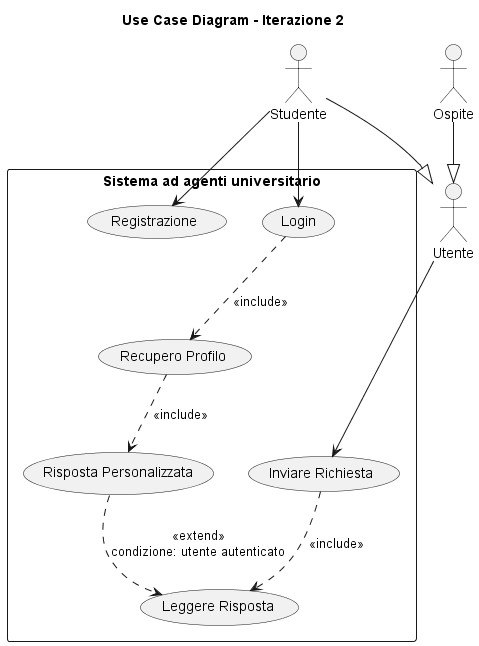
\includegraphics[width=0.85\textwidth]{usecase_diagram2}
\caption{Diagramma dei casi d'uso -- Iterazione 2}
\end{figure}

\section{Design dell'Architettura}

\subsection{Diagramma dei Componenti}

\begin{figure}[H]
\centering

\includegraphics[width=\textwidth]{component_diagram2}
\caption{Diagramma dei componenti -- Architettura a tre tier (Iterazione 2)}
\end{figure}

\begin{figure}[H]
\centering
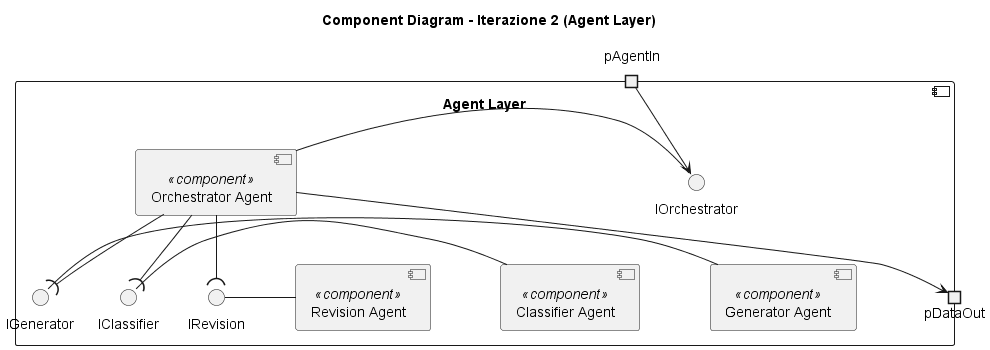
\includegraphics[width=0.85\textwidth]{component_agents_diagram2}
\caption{Diagramma dei componenti -- Agenti (Iterazione 2)}
\end{figure}

\begin{figure}[H]
\centering
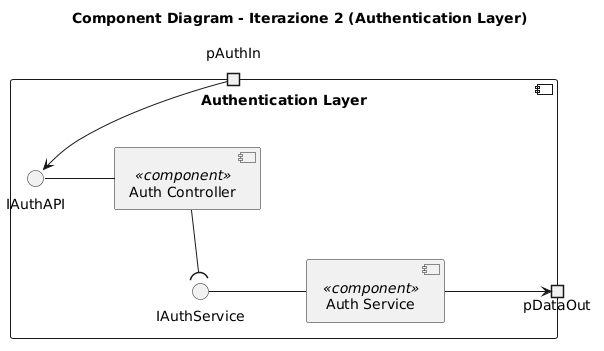
\includegraphics[width=0.85\textwidth]{component_auth_diagram2}
\caption{Diagramma dei componenti -- Layer Autenticazione (Iterazione 2)}
\end{figure}

\subsection{Diagramma delle Classi}

\begin{figure}[H]
\centering

\includegraphics[width=\textwidth]{class_diagram2}
\caption{Diagramma delle classi -- Iterazione 2}
\end{figure}

Il layer di autenticazione segue il pattern \textbf{Controller $\rightarrow$ Service $\rightarrow$ Repository}:
\begin{itemize}
    \item \texttt{AuthController}: ponte HTTP, gestione cookie, filtro campi sensibili
    \item \texttt{AuthService}: logica applicativa (authenticate, createUser), bcrypt
    \item \texttt{ProfileRepository}: CRUD su MongoDB (findById, save, exists)
    \item \texttt{JWTManager}: generazione/validazione token (predisposto, non ancora usato)
\end{itemize}

\subsection{Diagramma di Sequenza}

\begin{figure}[H]
\centering

\includegraphics[width=\textwidth]{sequence_diagram2}
\caption{Diagramma di sequenza -- Login e query personalizzata (Iterazione 2)}
\end{figure}

\subsection{Diagramma di Attività}

\begin{figure}[H]
\centering
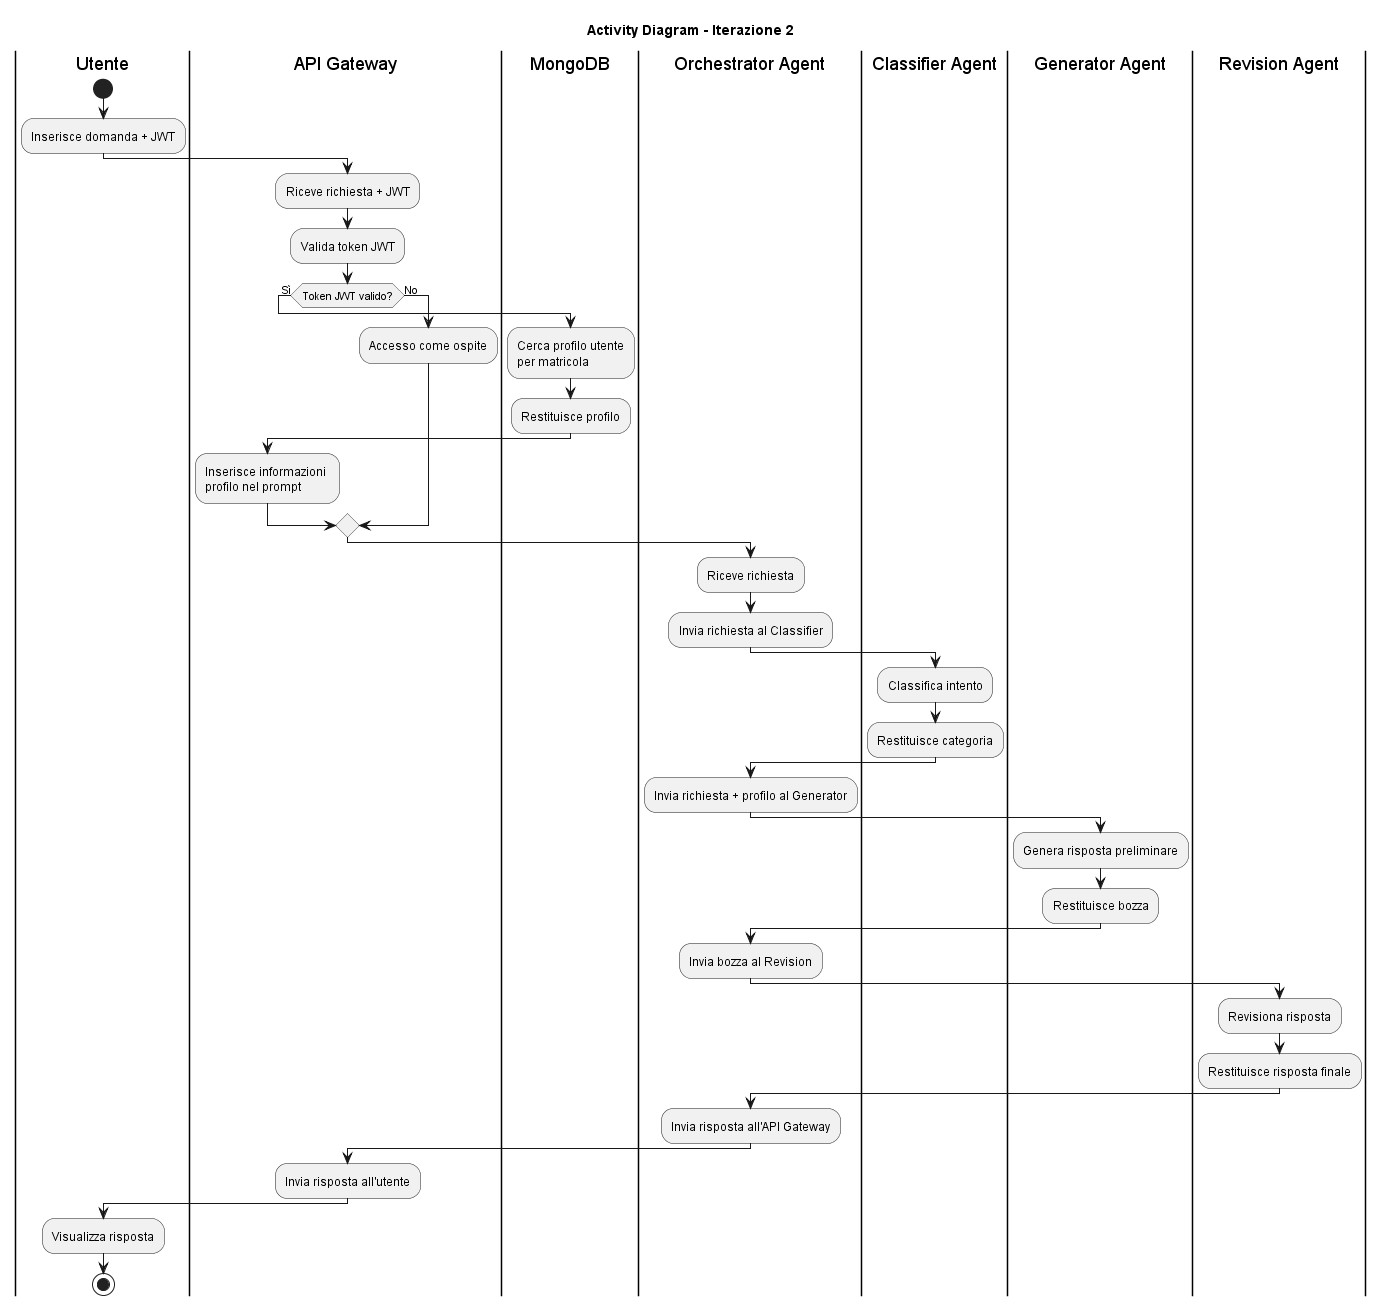
\includegraphics[width=0.75\textwidth]{activity_diagram2}
\caption{Diagramma di attività -- Flusso registrazione/login e query (Iterazione 2)}
\end{figure}

\subsection{Algoritmi e Complessità}

\paragraph{Autenticazione.}
Login: lookup per chiave indicizzata $O(D) = O(\log N)$ su B-tree MongoDB + \texttt{bcrypt.checkpw} $O(B) \approx 100$ms con cost factor 12. Totale: $O(D + B)$.

Registrazione: verifica unicità + hash + insert: $O(2D + B)$.

Il costo $O(B)$ di bcrypt è intenzionalmente elevato (design by intent) per resistere ad attacchi brute-force.

\paragraph{Costruzione contesto utente.}
\texttt{build\_user\_context(state)} concatena $p=8$ stringhe: $O(1)$ (costante). Chiamata una volta per nodo del grafo.

\section{Testing Dinamico}

\begin{table}[H]
\centering
\small
\begin{tabularx}{\textwidth}{l l l X l}
\toprule
\textbf{ID} & \textbf{Endpoint} & \textbf{Met.} & \textbf{Descrizione} & \textbf{Atteso} \\
\midrule
IT2-01 & \texttt{/api/auth/register} & POST & Registrazione nuovo studente & 200 \\
IT2-02 & \texttt{/api/auth/register} & POST & Matricola duplicata & 409 \\
IT2-03 & \texttt{/api/auth/login} & POST & Login credenziali corrette & 200 \\
IT2-04 & \texttt{/api/auth/login} & POST & Matricola inesistente & 401 \\
IT2-05 & \texttt{/api/auth/login} & POST & Password errata & 401 \\
IT2-06 & \texttt{/api/auth/verify} & GET & Token valido & 200 \\
IT2-07 & \texttt{/api/auth/verify} & GET & Senza cookie & 401 \\
IT2-08 & \texttt{/api/auth/profile} & PUT & Aggiornamento profilo & 200 \\
IT2-09 & \texttt{/api/auth/password} & PUT & Cambio password valido & 200 \\
IT2-10 & \texttt{/api/auth/password} & PUT & Password corrente errata & 401 \\
IT2-11 & \texttt{/api/agent/query} & POST & Query personalizzata & 200 \\
IT2-12 & \texttt{/api/auth/logout} & POST & Logout & 200 \\
\bottomrule
\end{tabularx}
\caption{Test API -- Iterazione 2 (12 test, 7 endpoint)}
\end{table}

\textbf{Setup Postman}: la variabile \texttt{jwt\_token} viene estratta automaticamente dal cookie \texttt{access\_token} nello script di test di IT2-01 e IT2-03, e riutilizzata nelle richieste successive.

\textbf{Asserzioni chiave}: il cookie \texttt{access\_token} è \texttt{httponly}; le risposte non contengono \texttt{passwordHash}; le query personalizzate utilizzano le informazioni del profilo.

\textbf{Esecuzione automatizzata}:
\begin{verbatim}
newman run postman_collection.json --folder "Iterazione 2"
\end{verbatim}

\section{Analisi Statica del Codice}

Con l'introduzione del pacchetto \texttt{auth/}, il codebase cresce significativamente. I nuovi moduli presentano:
\begin{itemize}
    \item \texttt{auth/controller.py}: CC = A (tutte le funzioni CC $\leq$ 1), MI = 100.00 (eccellente)
    \item \texttt{auth/service.py}: CC max = A (\texttt{authenticate}, CC=3), MI = 80.09
    \item \texttt{auth/profile\_repository.py}: CC max = A (\texttt{updateProfile}, CC=4), MI = 81.33
    \item \texttt{auth/jwt\_manager.py}: CC max = A (\texttt{\_\_init\_\_}, CC=2), MI = 86.28
    \item \texttt{models/user.py}: CC = A (tutte CC=1), MI = 100.00
\end{itemize}

Il layer Auth conferma un design pulito con responsabilità ben separate: tutti i metodi hanno complessità $\leq$ 4.


% ═══════════════════════════════════════════════════════════════════
% CHAPTER 5 – ITERAZIONE 3
% ═══════════════════════════════════════════════════════════════════
\chapter{Iterazione 3 -- JWT, Gestione Sessione e Memoria Conversazionale}

\section{Obiettivo dell'Iterazione}

Consolidare il sistema con tre macro-funzionalità:
\begin{itemize}
    \item \textbf{JWT Authentication via httpOnly Cookie}: token di sessione stateless, HMAC-SHA256, scadenza 7 giorni
    \item \textbf{Gestione della Sessione Browser}: ripristino automatico al ricaricamento tramite \texttt{GET /api/auth/verify}
    \item \textbf{Memoria Conversazionale}: cronologia in \texttt{localStorage}, trasmessa come \texttt{conversation\_history}
\end{itemize}

\subsection{Evoluzione rispetto all'Iterazione 2}

\begin{table}[H]
\centering
\small
\begin{tabularx}{\textwidth}{l X X}
\toprule
\textbf{Funzionalità} & \textbf{Iterazione 2} & \textbf{Iterazione 3} \\
\midrule
JWT & Assente & httpOnly cookie HMAC-SHA256 \\
Ripristino sessione & Assente & \texttt{GET /api/auth/verify} \\
Logout & Assente & \texttt{POST /api/auth/logout} + delete cookie \\
Memoria conversazionale & Assente & localStorage + conversation\_history \\
Auth Layer & Logica in main.py & Pacchetto \texttt{auth/} con 4 classi \\
CORS & \texttt{allow\_origins=["*"]} & Origini ristrette \\
\bottomrule
\end{tabularx}
\caption{Evoluzione dall'Iterazione 2 alla 3}
\end{table}

\section{Analisi dei Requisiti e Use Case}

\subsection{Use Case}

\begin{itemize}
    \item \textbf{UC-01 -- Registrazione} (aggiornato): al termine, \texttt{JWTManager.generateToken()} genera il token e \texttt{AuthController.\_set\_auth\_cookie()} imposta l'httpOnly cookie.

    \item \textbf{UC-02 -- Login} (aggiornato): \texttt{AuthService.authenticate()} verifica bcrypt $\rightarrow$ \texttt{JWTManager.generateToken()} $\rightarrow$ cookie impostato $\rightarrow$ frontend carica conversazione da localStorage.

    \item \textbf{UC-08 -- Ripristino Sessione Automatica}: al caricamento React, \texttt{GET /api/auth/verify} con \texttt{credentials: "include"} $\rightarrow$ backend decodifica JWT dal cookie $\rightarrow$ lookup MongoDB $\rightarrow$ profilo restituito $\rightarrow$ conversazione da localStorage. Flusso alternativo: token assente/scaduto $\rightarrow$ pagina login.

    \item \textbf{UC-09 -- Logout Sicuro}: \texttt{POST /api/auth/logout} $\rightarrow$ \texttt{response.delete\_cookie("access\_token")} $\rightarrow$ frontend rimuove profilo e localStorage $\rightarrow$ redirect login.

    \item \textbf{UC-10 -- Richiesta Contestuale}: il frontend include gli ultimi 10 messaggi (5 turni) nel body. Ogni agente usa la history in modo diverso:
    \begin{itemize}
        \item ClassifierAgent: ultimi 2 turni per disambiguare follow-up
        \item QueryAgent: ultimi 3 turni per query contestuali
        \item GeneratorAgent: history completa come messaggi LLM nativi (\texttt{HumanMessage}/\texttt{AIMessage})
        \item RevisionAgent: ultimi 2 turni per coerenza
    \end{itemize}
\end{itemize}

\subsection{Requisiti Non Funzionali}

\begin{itemize}
    \item \textbf{RNF-1}: JWT solo via httpOnly cookie; SameSite=lax
    \item \textbf{RNF-2}: scadenza JWT 7 giorni; alla scadenza $\rightarrow$ 401 e redirect login
    \item \textbf{RNF-3}: conversazione in localStorage con chiave \texttt{conversation\_\{matricola\}}
    \item \textbf{RNF-4}: al logout, pulizia completa (anche in caso di errore di rete)
    \item \textbf{RNF-5}: max 10 messaggi nella \texttt{conversation\_history}
    \item \textbf{RNF-6}: CORS con origini esplicite, \texttt{allow\_credentials=True}
    \item \textbf{RNF-7}: auth layer nel pacchetto \texttt{auth/} separato da \texttt{main.py}
    \item \textbf{RNF-8}: verify entro 2 secondi; pipeline entro 15 secondi
\end{itemize}

\begin{figure}[H]
\centering
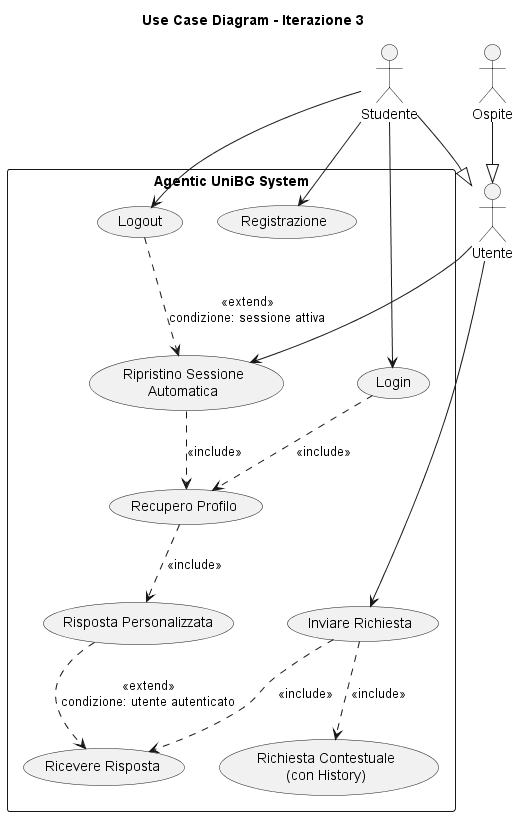
\includegraphics[width=0.85\textwidth]{usecase_diagram3}
\caption{Diagramma dei casi d'uso -- Iterazione 3}
\end{figure}

\section{Design dell'Architettura}

\subsection{Diagramma dei Componenti}

\begin{figure}[H]
\centering
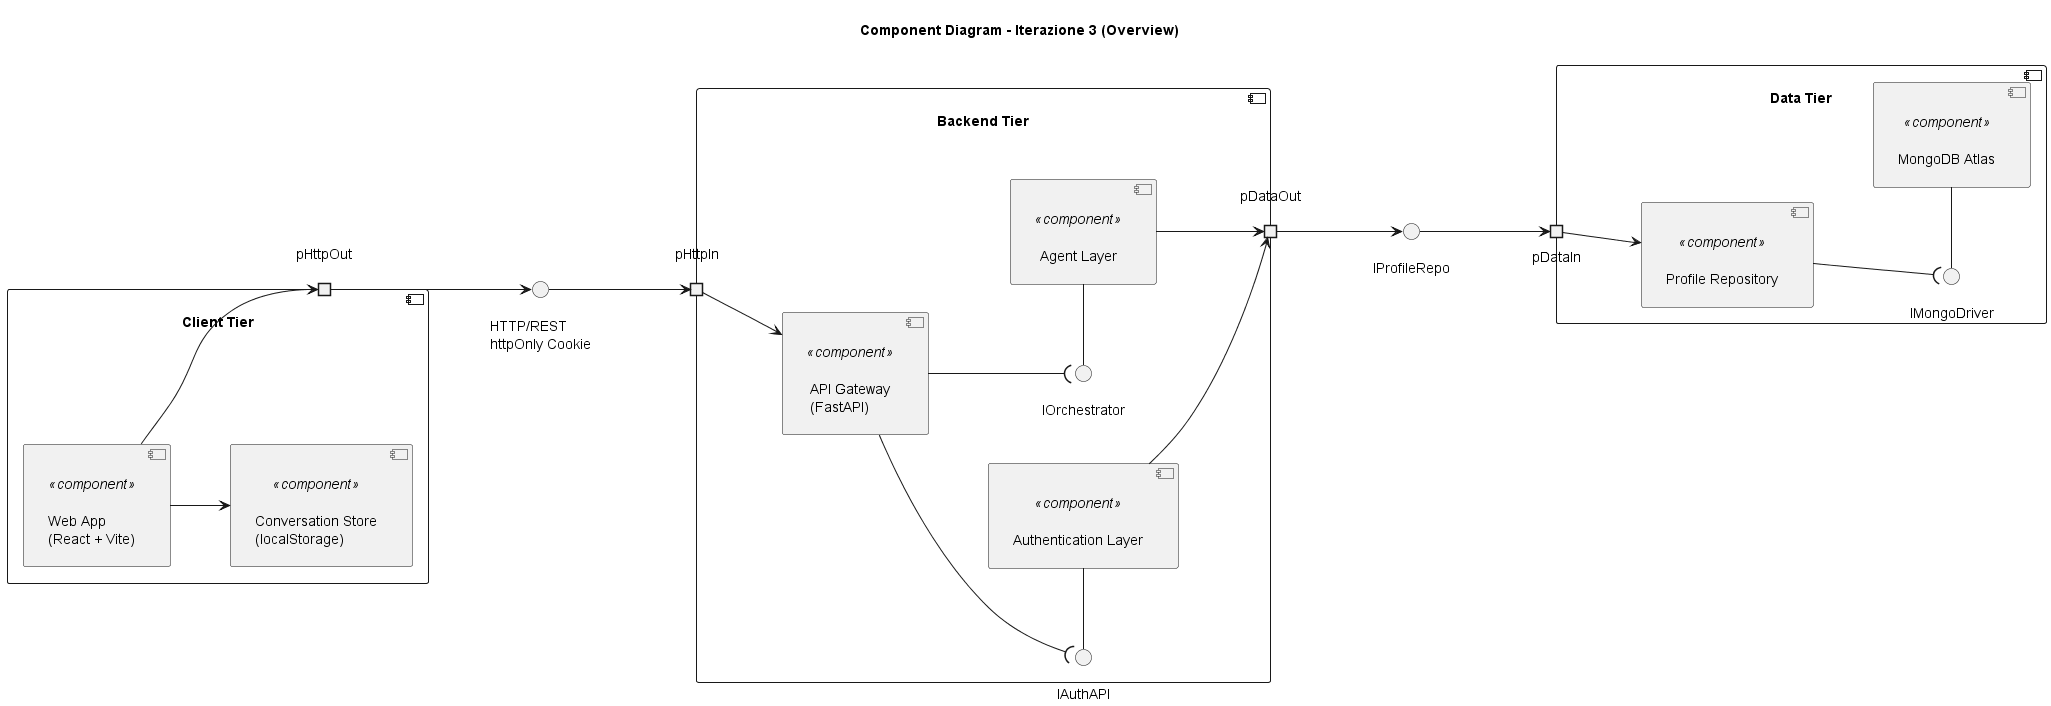
\includegraphics[width=\textwidth]{component_diagram3}
\caption{Diagramma dei componenti -- Architettura completa (Iterazione 3)}
\end{figure}

\begin{figure}[H]
\centering
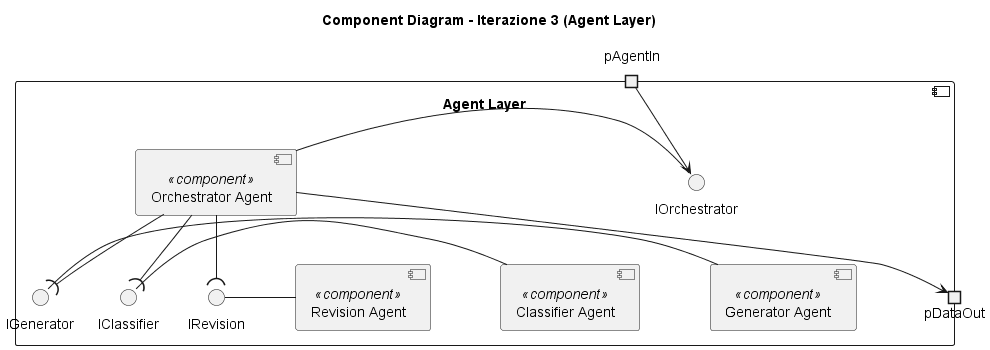
\includegraphics[width=0.85\textwidth]{component_agents_diagram3}
\caption{Diagramma dei componenti -- Agenti (Iterazione 3)}
\end{figure}

\subsubsection{Alternative di Design: Persistenza Conversazione}

Sono state valutate tre alternative per la persistenza della memoria conversazionale:

\begin{figure}[H]
\centering
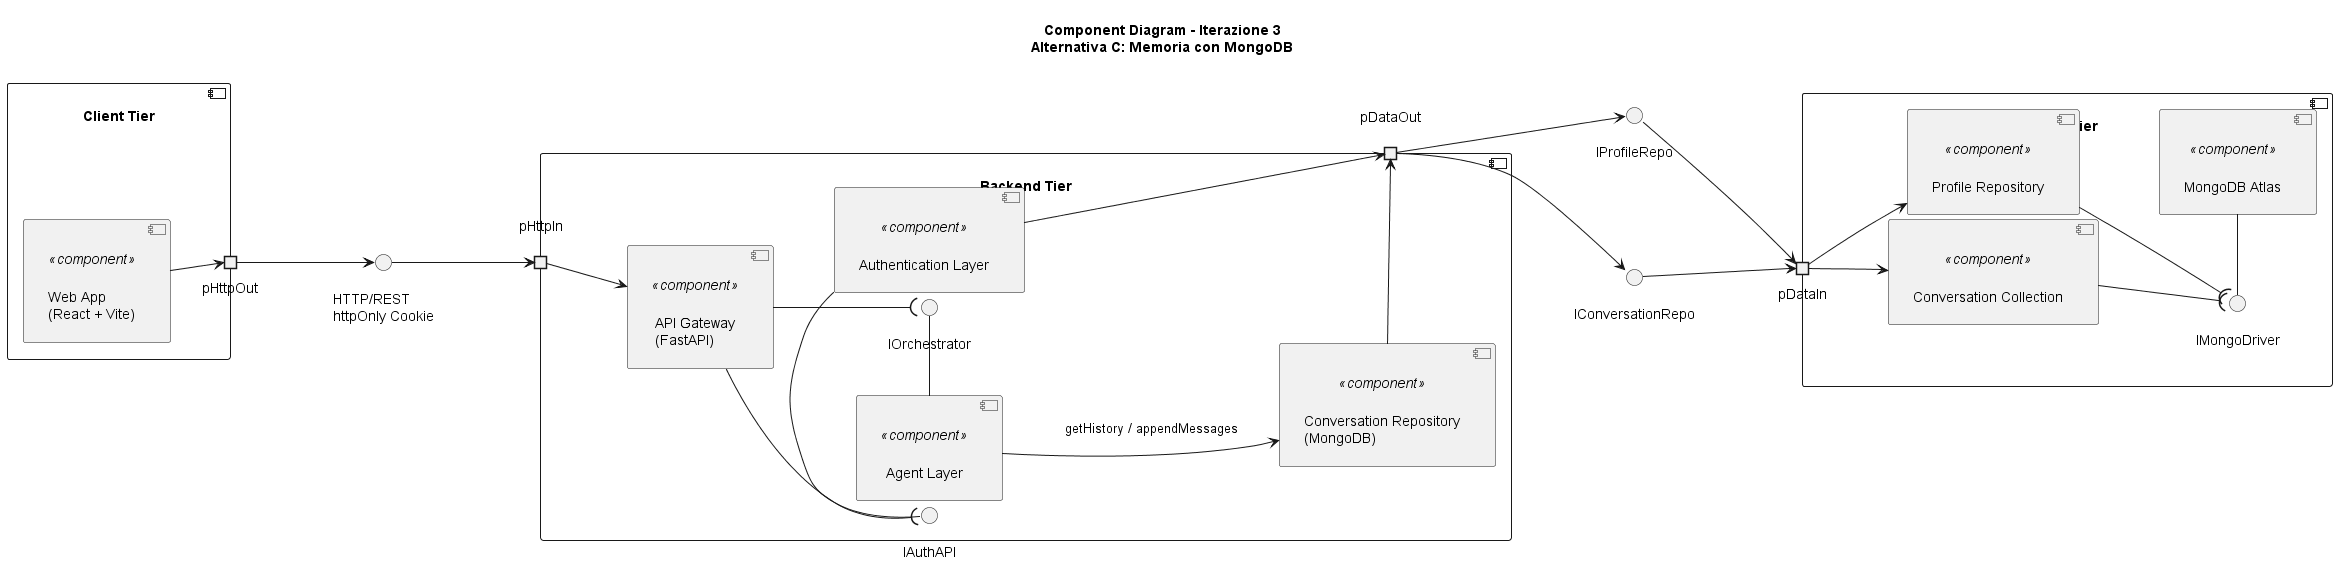
\includegraphics[width=0.85\textwidth]{component3_mongodb}
\caption{Alternativa C -- Persistenza conversazione su MongoDB}
\end{figure}

\begin{figure}[H]
\centering
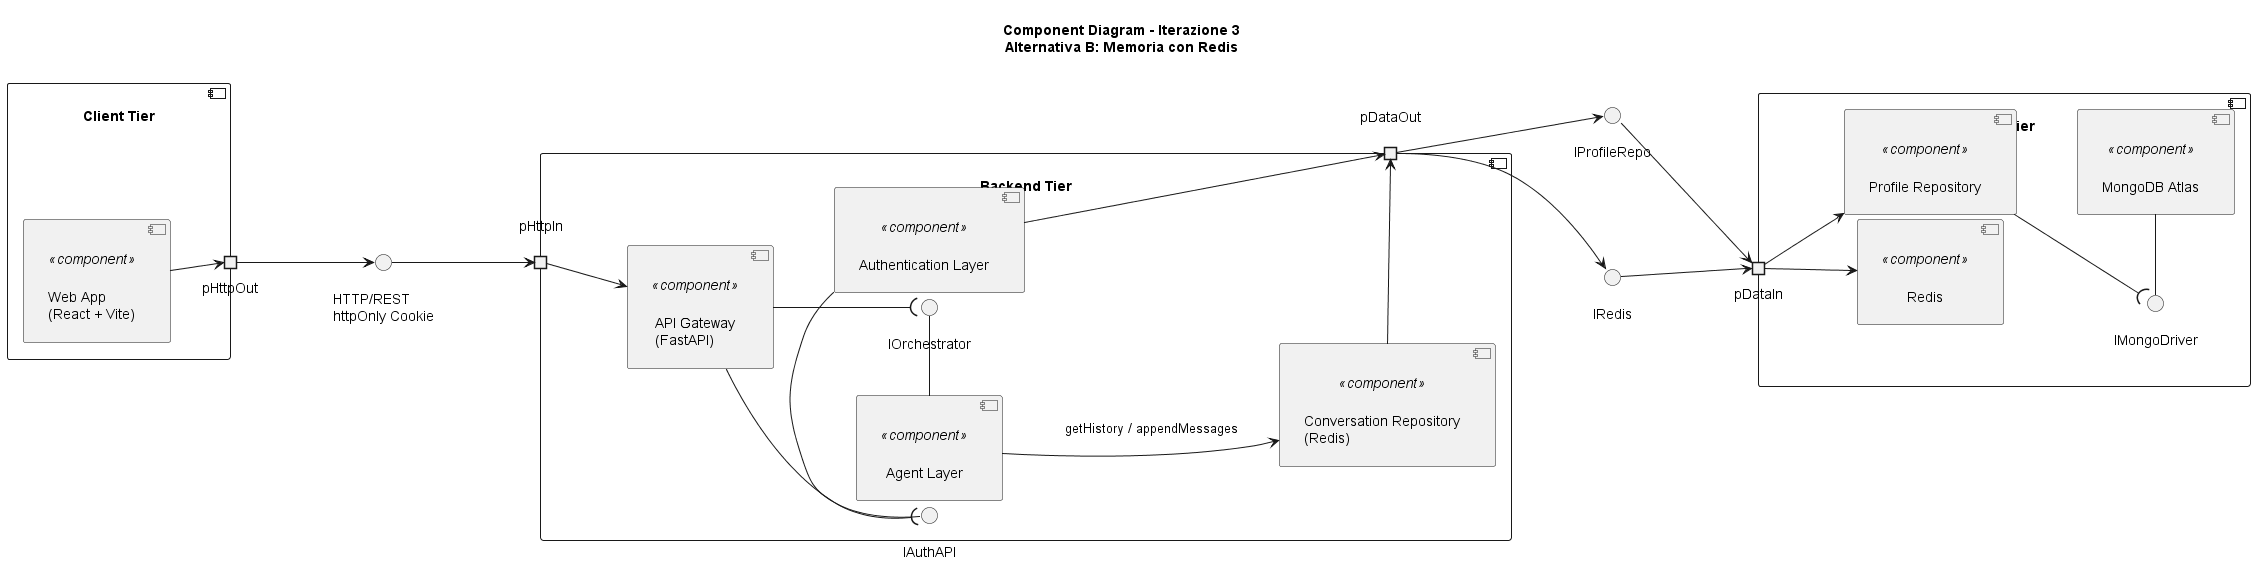
\includegraphics[width=0.85\textwidth]{component3_redis}
\caption{Alternativa B -- Persistenza conversazione su Redis}
\end{figure}

\begin{table}[H]
\centering
\small
\begin{tabularx}{\textwidth}{l X l}
\toprule
\textbf{Alternativa} & \textbf{Descrizione} & \textbf{Scelta} \\
\midrule
A -- localStorage & History lato client, max 10 msg, nessun server storage & \textbf{Implementata} \\
B -- Redis & History server con TTL 24h, flush su MongoDB al logout & Scartata \\
C -- MongoDB & History permanente su DB, multi-conversazione & Scartata \\
\bottomrule
\end{tabularx}
\caption{Alternative di design -- Memoria conversazionale}
\end{table}

Scelta motivata dalla semplicità e adeguatezza per il caso d'uso, in linea con il principio AMDD ``just enough modeling''.

\subsection{Diagramma delle Classi}

\begin{figure}[H]
\centering
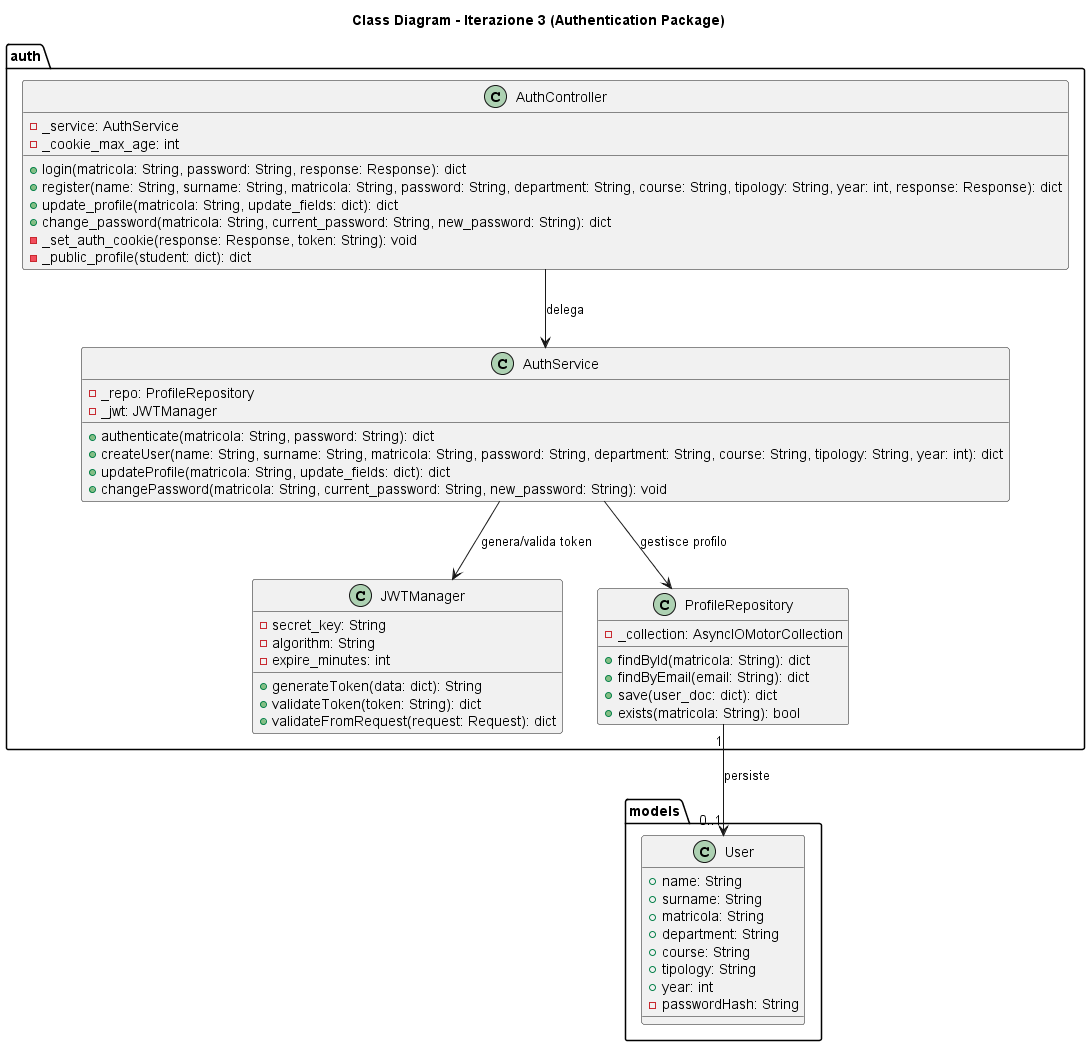
\includegraphics[width=0.9\textwidth]{class_auth_diagram3}
\caption{Diagramma delle classi -- Layer Autenticazione (Iterazione 3)}
\end{figure}

\begin{figure}[H]
\centering
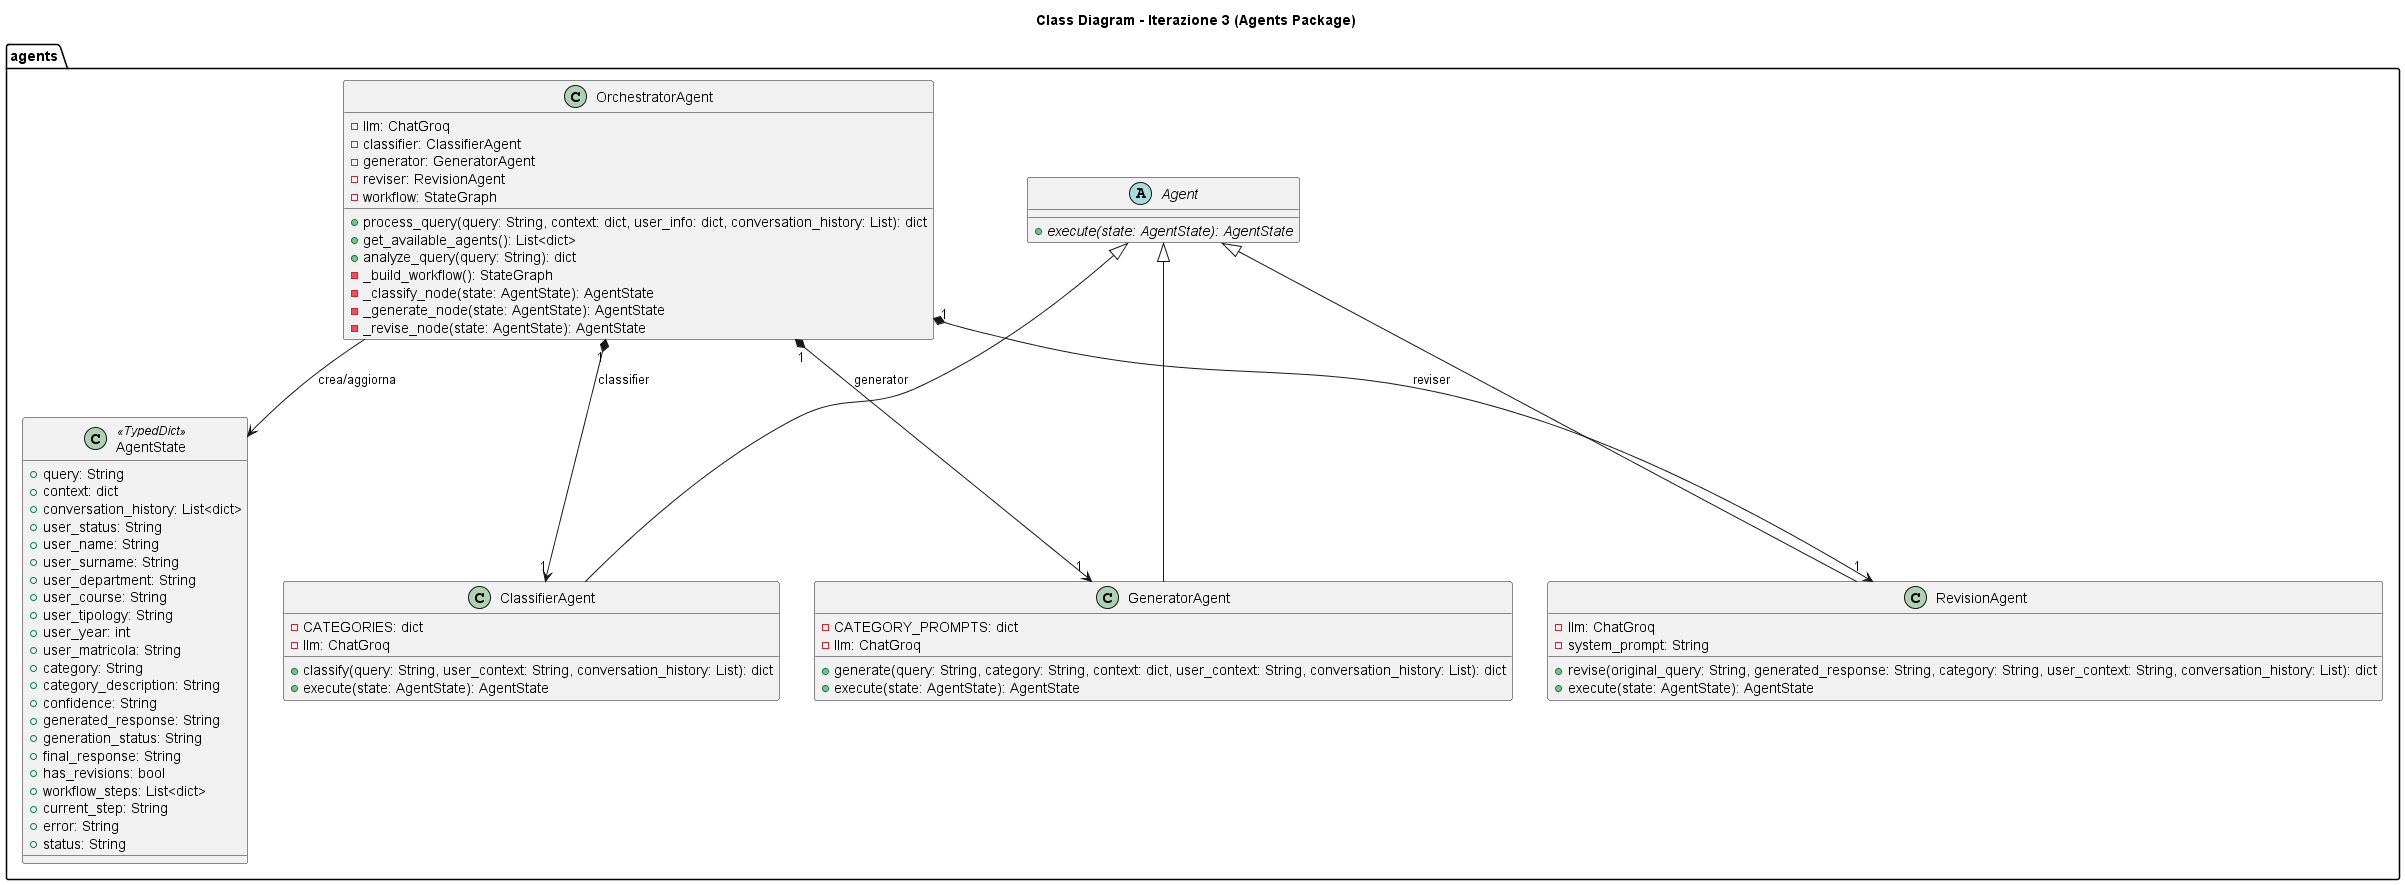
\includegraphics[width=0.9\textwidth]{class_agents_diagram3}
\caption{Diagramma delle classi -- Agenti (Iterazione 3)}
\end{figure}

\begin{figure}[H]
\centering
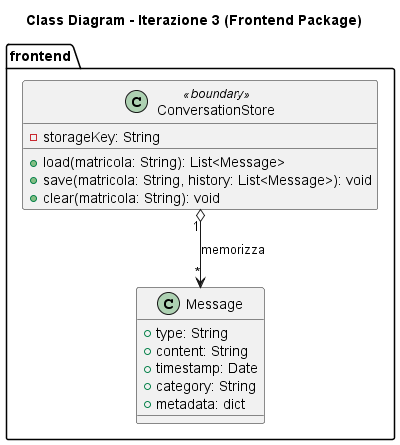
\includegraphics[width=0.8\textwidth]{class_frontend_diagram3}
\caption{Diagramma delle classi -- Frontend React (Iterazione 3)}
\end{figure}

\subsection{Diagramma di Sequenza}

\begin{figure}[H]
\centering
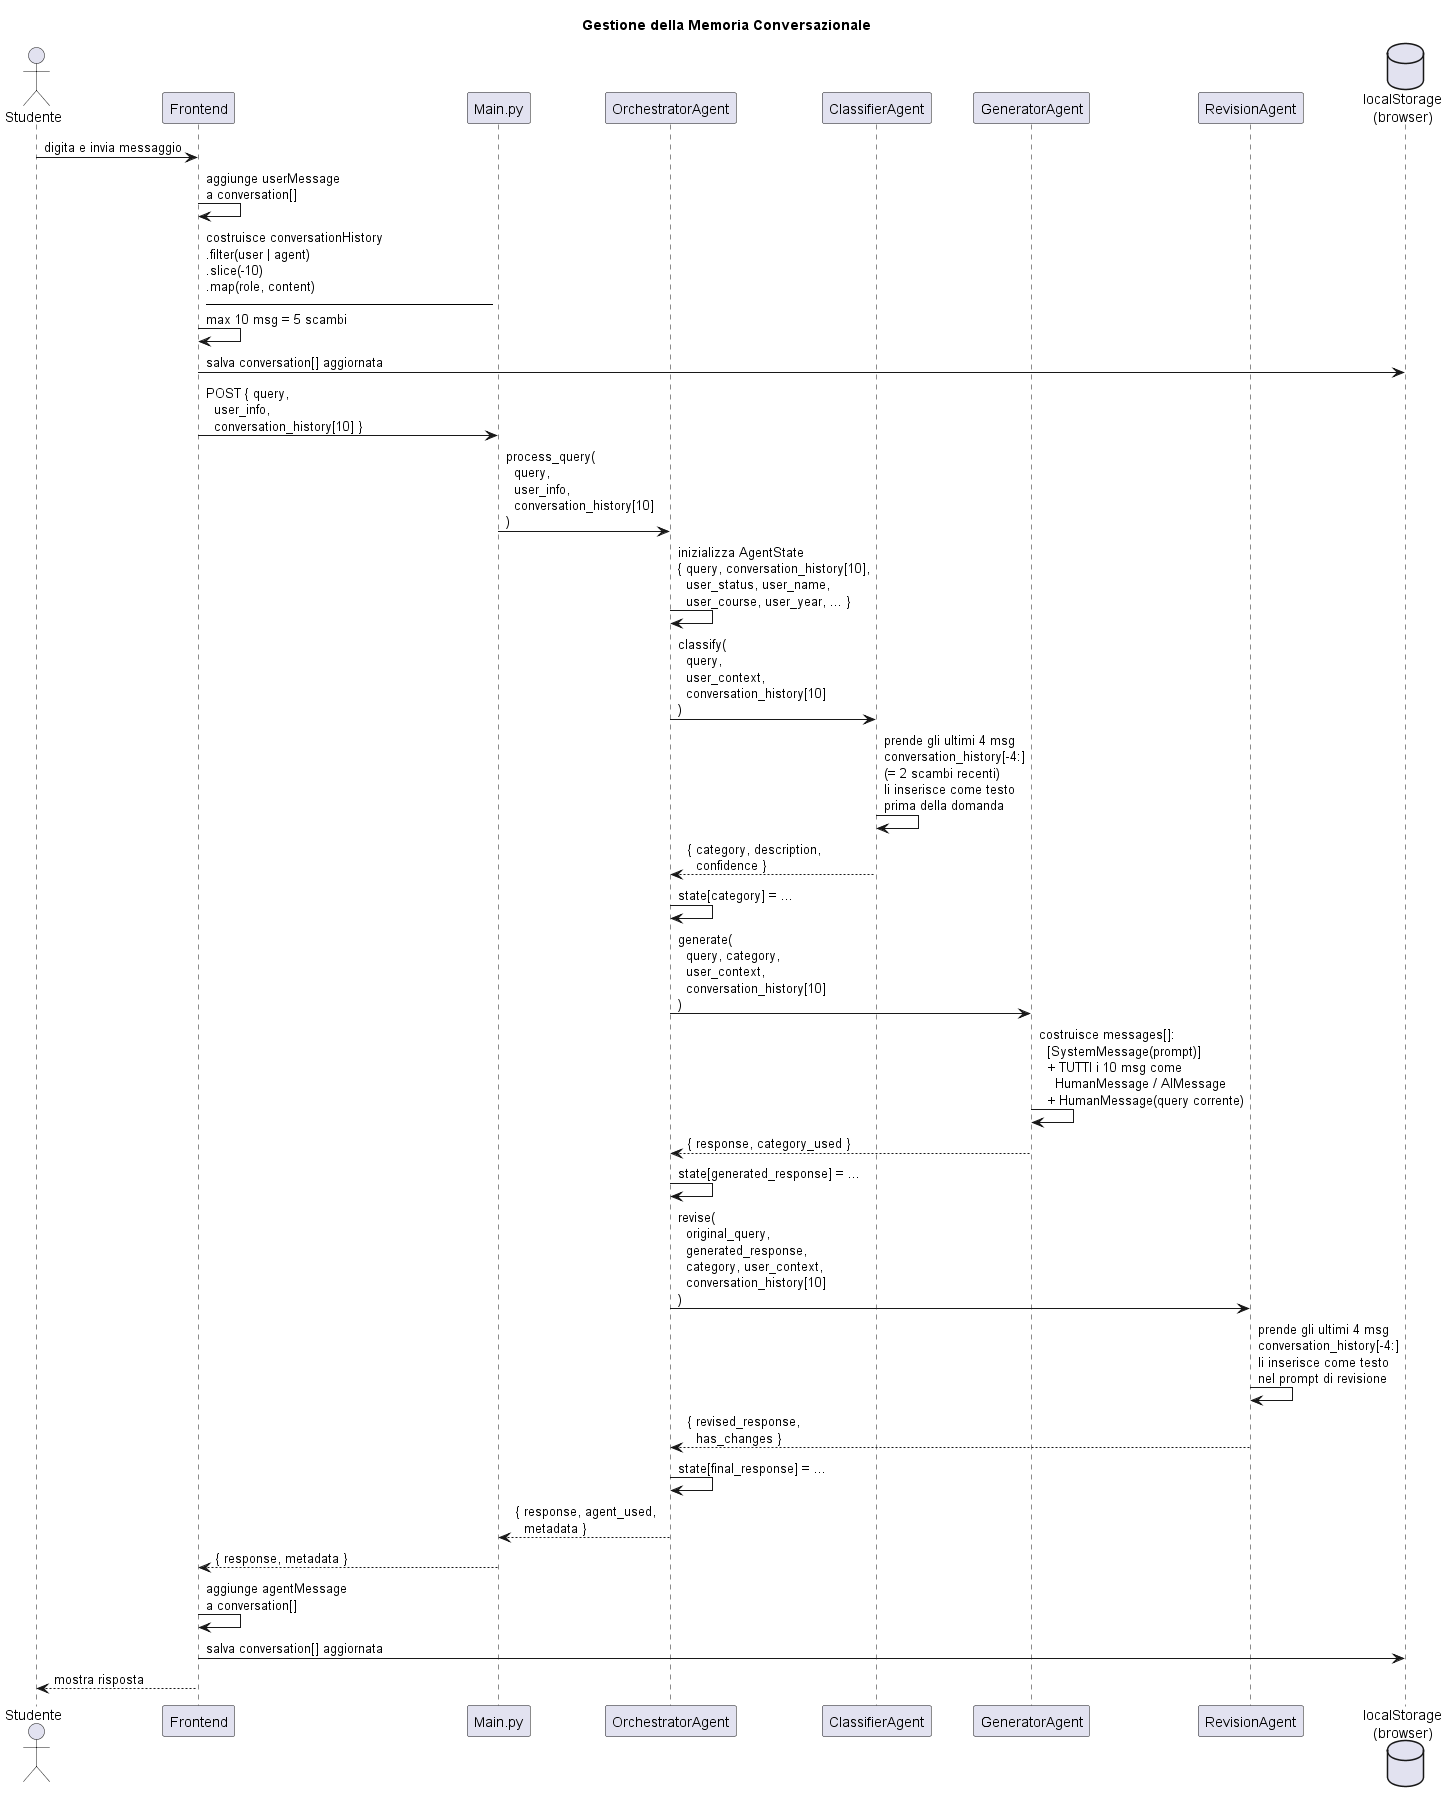
\includegraphics[width=\textwidth]{sequence_memory_diagram3}
\caption{Diagramma di sequenza -- Query con memoria conversazionale (Iterazione 3)}
\end{figure}

\begin{figure}[H]
\centering
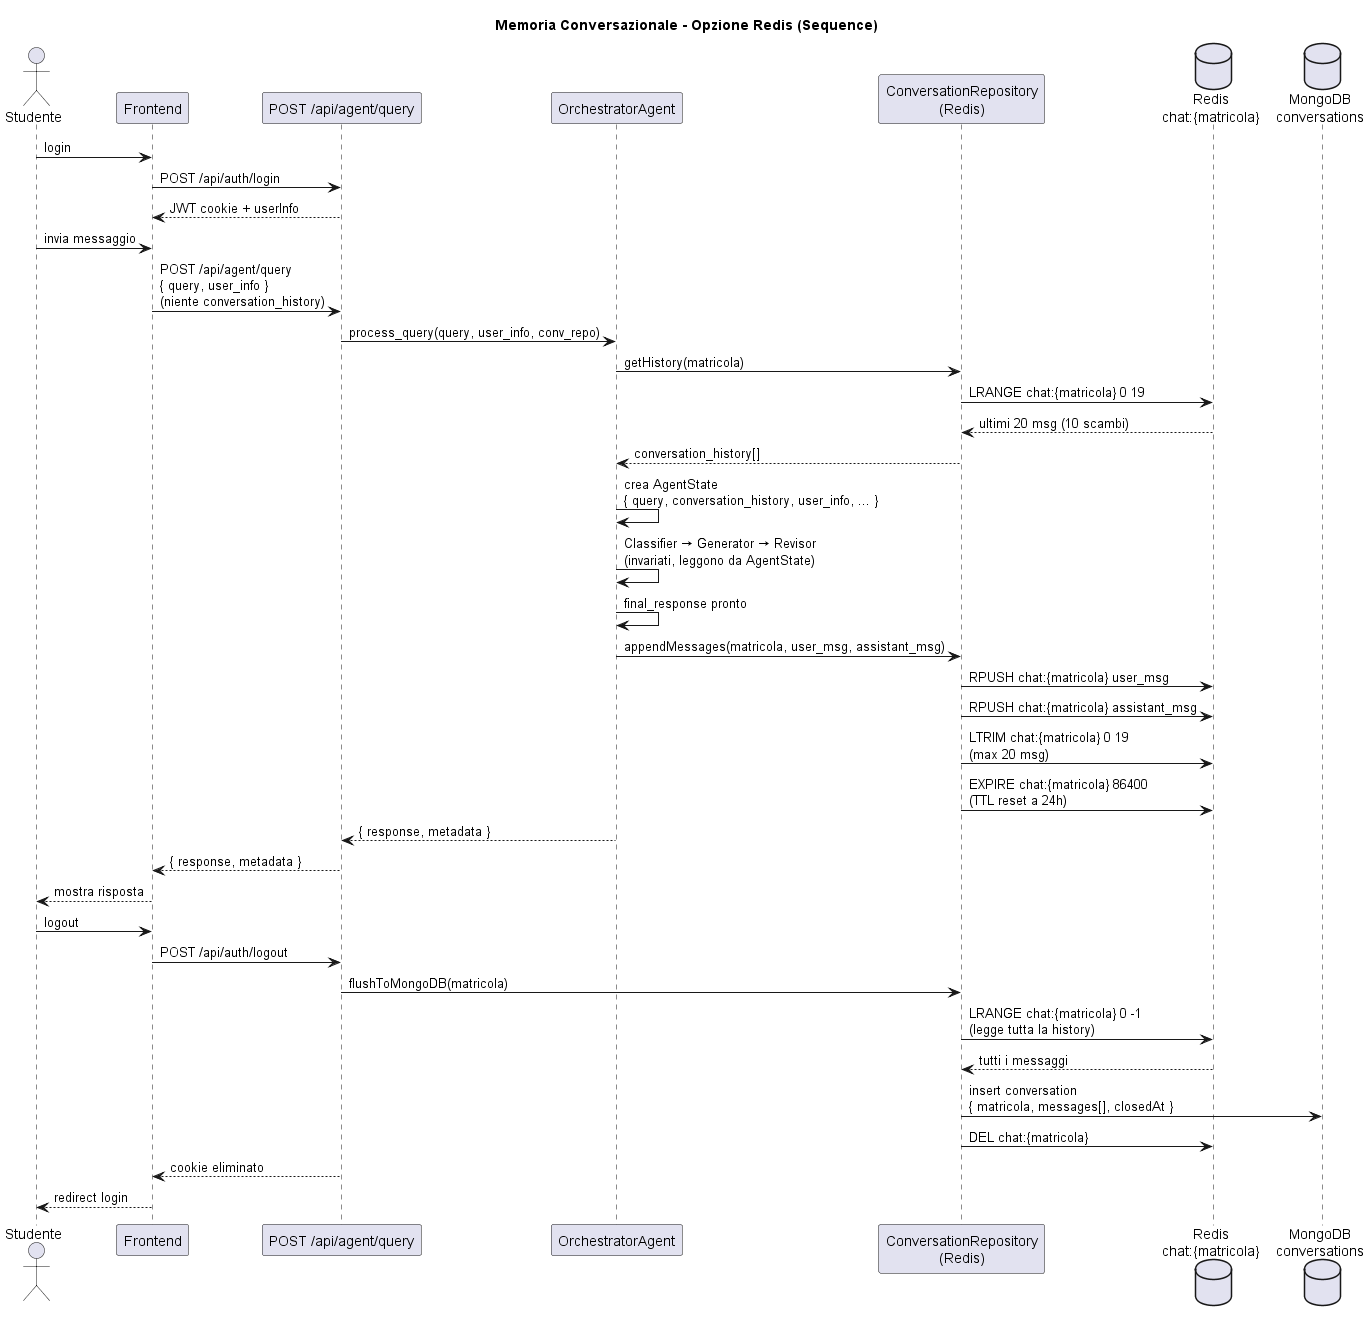
\includegraphics[width=\textwidth]{sequence_redis3}
\caption{Diagramma di sequenza -- Alternativa Redis (scartata)}
\end{figure}

\subsection{Diagramma di Attività}

\begin{figure}[H]
\centering
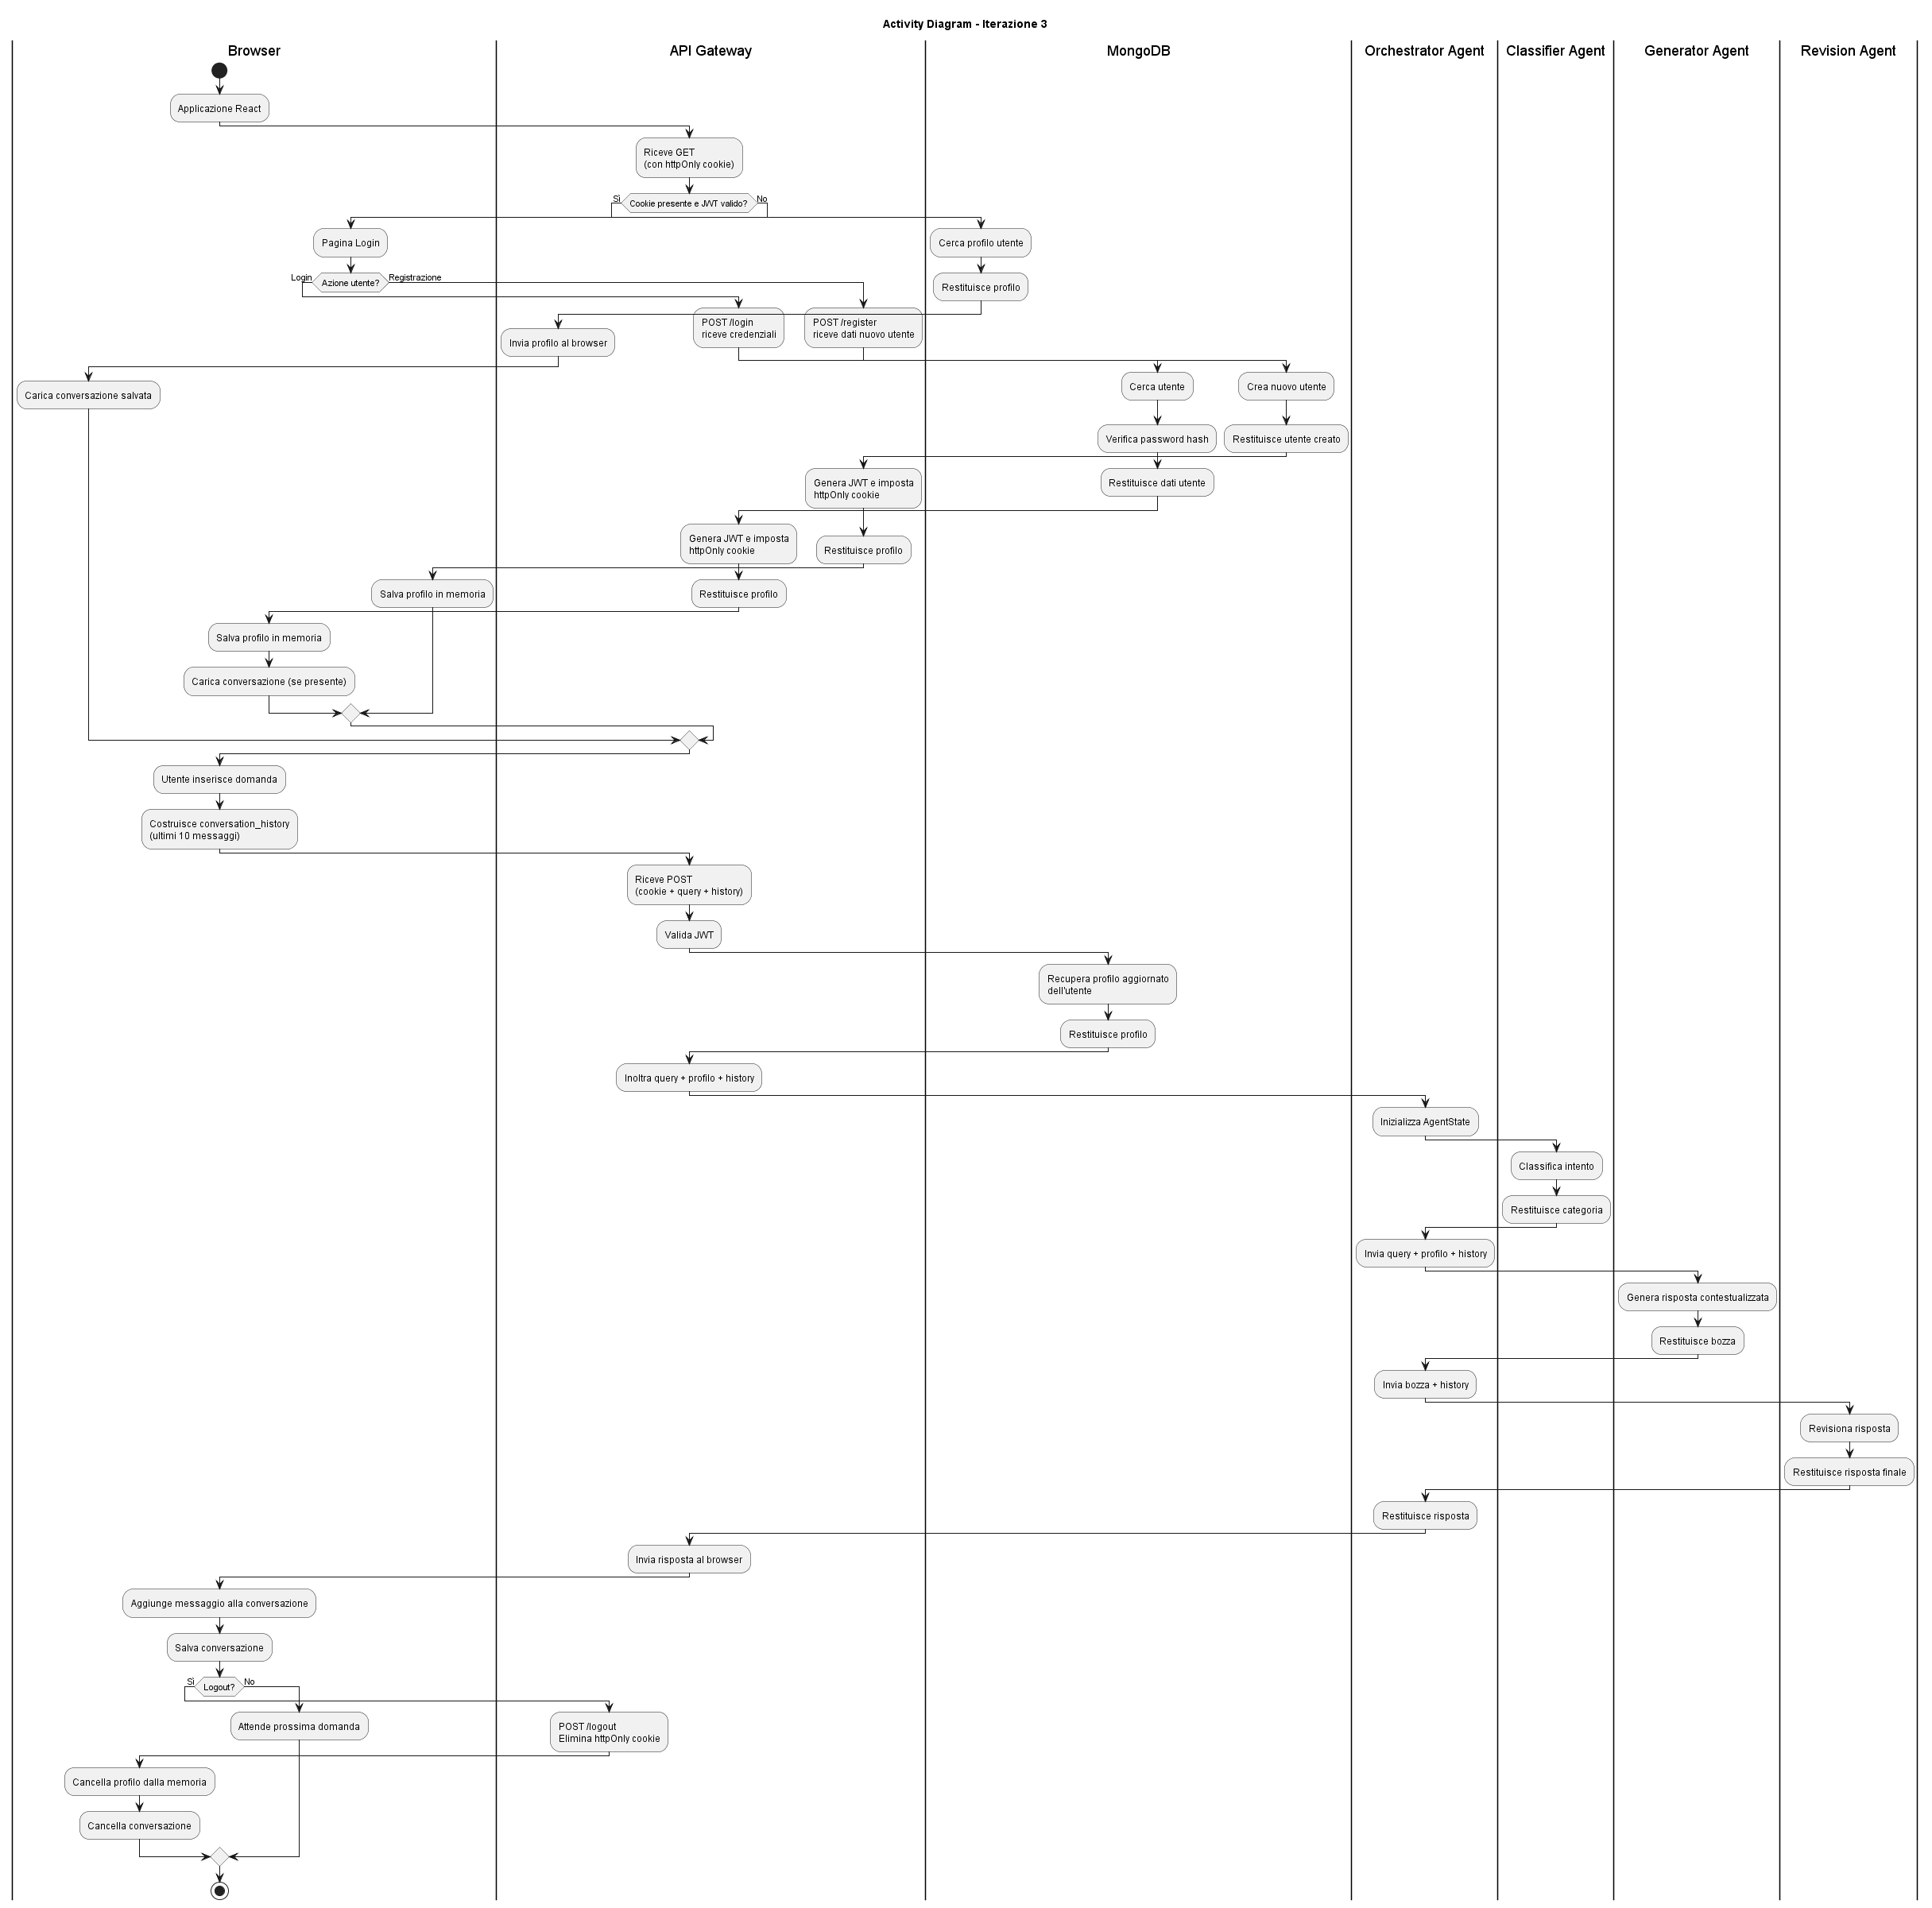
\includegraphics[width=0.75\textwidth]{activity_diagram3}
\caption{Diagramma di attività -- Flusso completo con sessione e memoria (Iterazione 3)}
\end{figure}

\subsection{Algoritmi e Complessità}

\paragraph{Contesto conversazionale nella pipeline.}
Il frontend filtra e seleziona gli ultimi $W=10$ messaggi ($O(H)$ dove $H$ è la dimensione totale della cronologia). Il costo della pipeline con contesto è $O(H + L(T))$ dove $L(T)$ è il costo LLM dipendente dal numero di token $T$ nella history troncata. La finestra di 10 messaggi limita $T$ e impedisce crescita lineare del costo.

\paragraph{Auto-verifica sessione.}
\texttt{GET /api/auth/verify}: $O(N_{net} + D + H)$ dove $N_{net}$ è la latenza di rete, $D$ il lookup MongoDB, $H$ il parsing di localStorage. La decodifica JWT è $O(1)$ (HMAC su payload fisso).

\section{Testing Dinamico}

\begin{table}[H]
\centering
\small
\begin{tabularx}{\textwidth}{l l l X l}
\toprule
\textbf{ID} & \textbf{Endpoint} & \textbf{Met.} & \textbf{Descrizione} & \textbf{Atteso} \\
\midrule
IT3-01 & \texttt{/api/agent/query} & POST & Prima domanda senza storico & 200 \\
IT3-02 & \texttt{/api/agent/query} & POST & Follow-up con contesto & 200 \\
IT3-03 & \texttt{/api/agent/query} & POST & Cambio argomento & 200 \\
IT3-04 & \texttt{/api/conversation/history} & GET & Recupero cronologia & 200 \\
IT3-05 & \texttt{/api/conversation/history} & DELETE & Cancellazione cronologia & 200 \\
\bottomrule
\end{tabularx}
\caption{Test API -- Iterazione 3 (5 test, 2 endpoint)}
\end{table}

\textbf{Asserzioni chiave}: il sistema disambigua domande di follow-up (es.\ ``E quelli di informatica?'') usando la \texttt{conversation\_history}; un cambio di argomento viene gestito senza confusione.

\textbf{Esecuzione automatizzata}:
\begin{verbatim}
newman run postman_collection.json --folder "Iterazione 3"
\end{verbatim}

\section{Analisi Statica del Codice}

Il refactoring del layer auth introduce il pacchetto \texttt{auth/} con 4 classi ben separate. L'impatto sulle metriche:

\begin{itemize}
    \item La complessità ciclomatica del layer auth resta in grado \textbf{A} (CC $\leq$ 4)
    \item L'estrazione da \texttt{main.py} migliora la manutenibilità di quest'ultimo
    \item L'\texttt{AgentState} acquisisce il campo \texttt{conversation\_history} senza impatto sulla CC
    \item Tutti i moduli mantengono MI grado \textbf{A}
\end{itemize}


% ═══════════════════════════════════════════════════════════════════
% CHAPTER 6 – ITERAZIONE 4
% ═══════════════════════════════════════════════════════════════════
\chapter{Iterazione 4 -- Web Search, Date Esami e Pipeline Logging}

\section{Obiettivo dell'Iterazione}

Arricchire il sistema con la capacità di recuperare informazioni reali e aggiornate dal sito dell'ateneo:
\begin{itemize}
    \item \textbf{QueryAgent}: generazione di query di ricerca web ottimizzate
    \item \textbf{WebAgent}: ricerca web tramite Tavily API su domini \texttt{unibg.it}
    \item \textbf{Categoria \texttt{date\_esami} con routing condizionale}: flusso dedicato per date esami con selezione intelligente del calendario
    \item \textbf{PipelineLogger}: logging strutturato su file
    \item \textbf{Cambio LLM}: da Groq / LLaMA 3.3 70B a Google Gemini 2.5 Flash
\end{itemize}

\subsection{Evoluzione rispetto all'Iterazione 3}

\begin{table}[H]
\centering
\small
\begin{tabularx}{\textwidth}{l X X}
\toprule
\textbf{Funzionalità} & \textbf{Iterazione 3} & \textbf{Iterazione 4} \\
\midrule
Recupero dati reali & Assente (solo LLM) & WebAgent su Tavily \\
Ottimizzazione query & Assente & QueryAgent con Gemini \\
Gestione PDF & Assente & WebAgent + PyMuPDF \\
Logging pipeline & Assente & PipelineLogger su file system \\
LLM Provider & Groq / LLaMA 3.3 70B & Google Gemini 2.5 Flash \\
Workflow & classify $\rightarrow$ generate $\rightarrow$ revise & classify $\rightarrow$ query $\rightarrow$ [web\_search $|$ exam\_extract] $\rightarrow$ generate $\rightarrow$ revise \\
Classificazione & 6 categorie & 7 categorie (+ date\_esami) \\
Routing & Lineare & Condizionale \\
\bottomrule
\end{tabularx}
\caption{Evoluzione dall'Iterazione 3 alla 4}
\end{table}

\section{Analisi dei Requisiti e Use Case}

\subsection{Use Case}

\begin{itemize}
    \item \textbf{UC-11 -- Risposta con Dati Reali da UniBG}: classify $\rightarrow$ QueryAgent (6-8 keyword) $\rightarrow$ WebAgent Tavily search (advanced, max 30) $\rightarrow$ top 5 + PyMuPDF PDF links $\rightarrow$ GeneratorAgent con web\_context $\rightarrow$ RevisionAgent $\rightarrow$ PipelineLogger.

    \item \textbf{UC-12 -- Logging Diagnostico}: ogni esecuzione genera un file \texttt{log\_\{matricola\}\_\{timestamp\}.txt} con: header, user info, query, history, step 1-5 (prompt + risposta), tempi.

    \item \textbf{UC-13 -- Risposta su Date Esami}: ClassifierAgent $\rightarrow$ \texttt{date\_esami} $\rightarrow$ routing condizionale $\rightarrow$ \texttt{exam\_extract}: LLM seleziona calendario da \texttt{EXAM\_CALENDAR\_LINKS} (4 poli $\times$ 4 sessioni) $\rightarrow$ Tavily Extract $\rightarrow$ ricerca aggiuntiva (top 3) $\rightarrow$ contesto combinato al GeneratorAgent. Ospite senza corso $\rightarrow$ \texttt{NUMERO: 0}.
\end{itemize}

\subsection{Requisiti Non Funzionali}

\begin{itemize}
    \item \textbf{RNF-1}: ricerca limitata a \texttt{unibg.it} e \texttt{unibg.coursecatalogue.cineca.it}
    \item \textbf{RNF-2}: latenza totale $\leq$ 30s; web search $\leq$ 10s
    \item \textbf{RNF-3}: fallback su risultati parziali se Tavily fallisce
    \item \textbf{RNF-4}: gestione PDF opzionale (graceful fallback se PyMuPDF non disponibile)
    \item \textbf{RNF-5}: log non bloccante (errori di scrittura ingoiati silenziosamente)
    \item \textbf{RNF-6}: context window $\leq$ 1M token (Gemini); selezione top 5 risultati
    \item \textbf{RNF-7}: query ottimizzata 6-8 termini
    \item \textbf{RNF-8}: cambio LLM provider trasparente
    \item \textbf{RNF-9--11}: ereditati (sicurezza bcrypt, JWT httpOnly, CORS origini esplicite)
    \item \textbf{RNF-12}: routing condizionale \texttt{date\_esami} $\rightarrow$ \texttt{exam\_extract}
    \item \textbf{RNF-13}: selezione calendario via LLM con fallback
\end{itemize}

\begin{figure}[H]
\centering
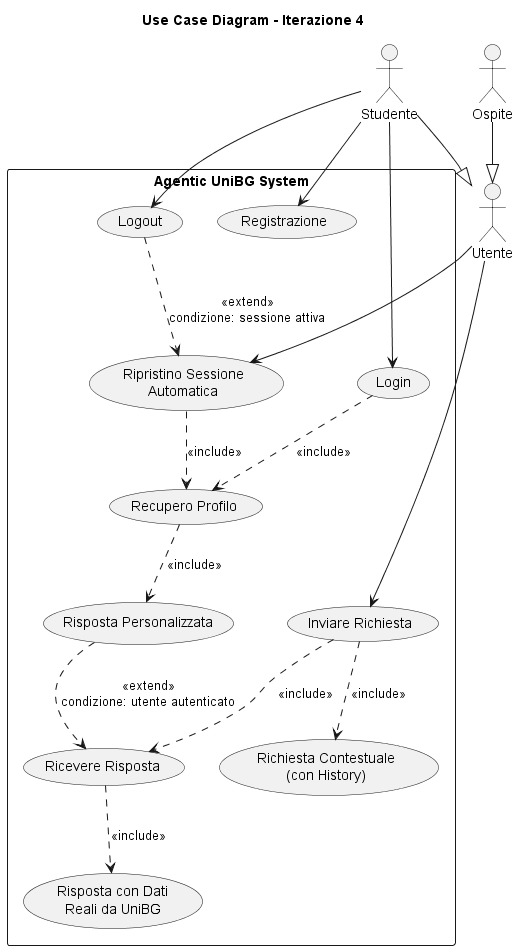
\includegraphics[width=0.85\textwidth]{usecase_diagram4}
\caption{Diagramma dei casi d'uso -- Iterazione 4}
\end{figure}

\section{Design dell'Architettura}

\subsection{Diagramma dei Componenti}

\begin{figure}[H]
\centering
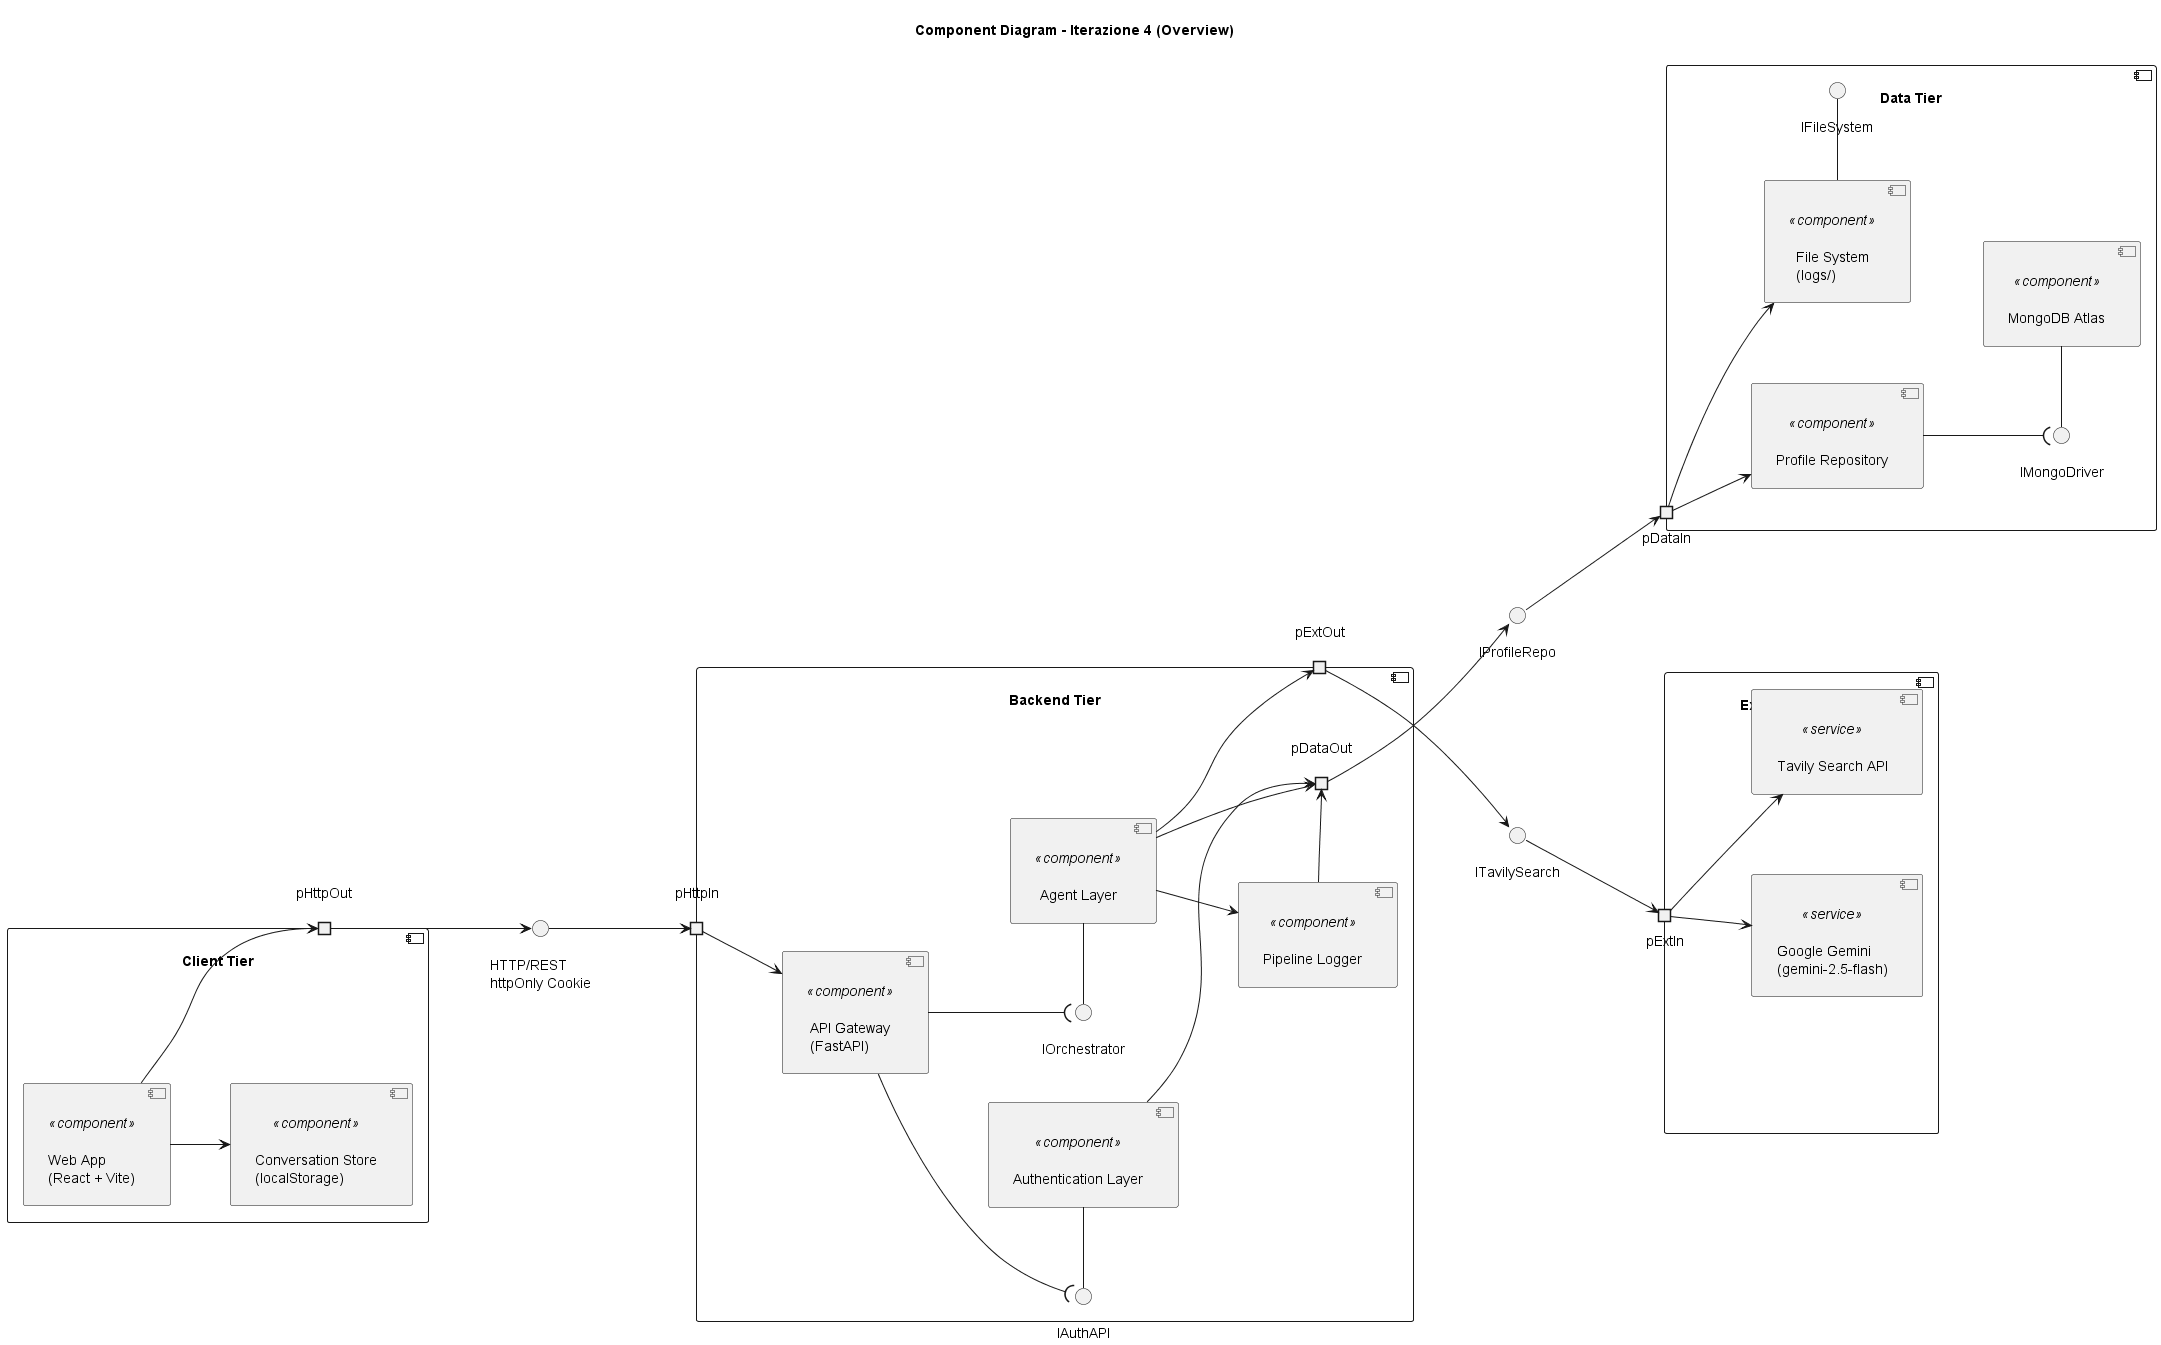
\includegraphics[width=\textwidth]{component4}
\caption{Diagramma dei componenti -- Architettura completa (Iterazione 4)}
\end{figure}

\begin{figure}[H]
\centering
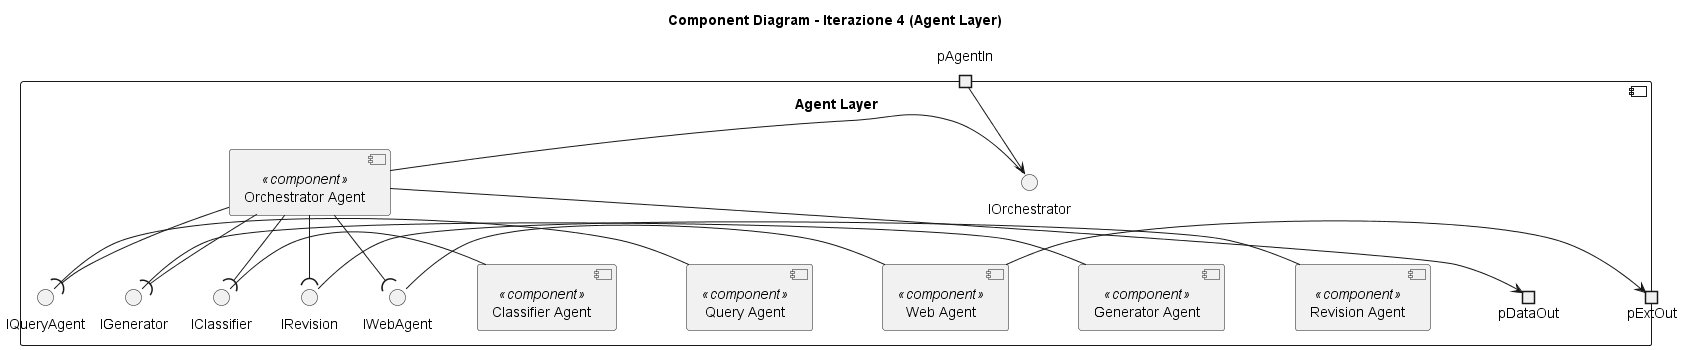
\includegraphics[width=0.85\textwidth]{component_agents_diagram4}
\caption{Diagramma dei componenti -- Agenti con routing condizionale (Iterazione 4)}
\end{figure}

\begin{figure}[H]
\centering
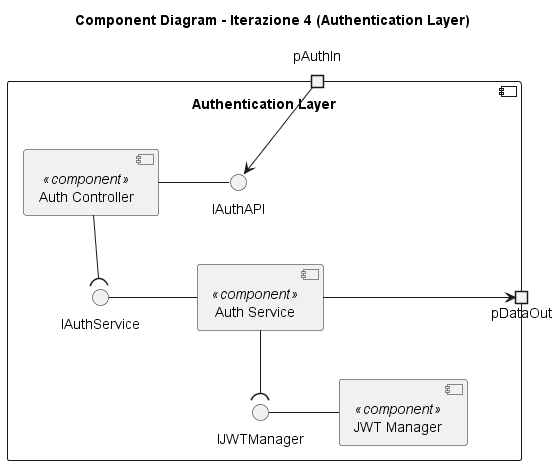
\includegraphics[width=0.85\textwidth]{component_auth_diagram4}
\caption{Diagramma dei componenti -- Layer Autenticazione (Iterazione 4)}
\end{figure}

\begin{figure}[H]
\centering
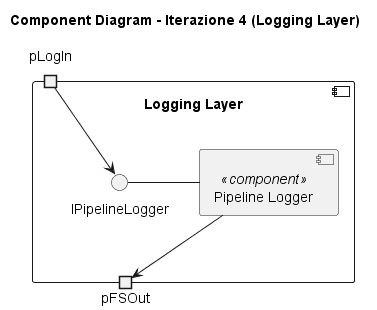
\includegraphics[width=0.85\textwidth]{component_logging_diagram4}
\caption{Diagramma dei componenti -- PipelineLogger (Iterazione 4)}
\end{figure}

\subsubsection{Workflow LangGraph}

Il workflow include un \textbf{branch condizionale} dopo il nodo \texttt{query}:

\begin{verbatim}
classify → query → [routing condizionale] → generate → revise → END
                     ├── web_search      (tutte le categorie)
                     └── exam_extract    (solo date_esami)
\end{verbatim}

Il metodo \texttt{\_route\_after\_query(state)} verifica \texttt{state["category"] == "date\_esami"} e instrada il flusso. Entrambi i rami convergono su \texttt{generate}.

\subsection{Diagramma delle Classi}

\begin{figure}[H]
\centering
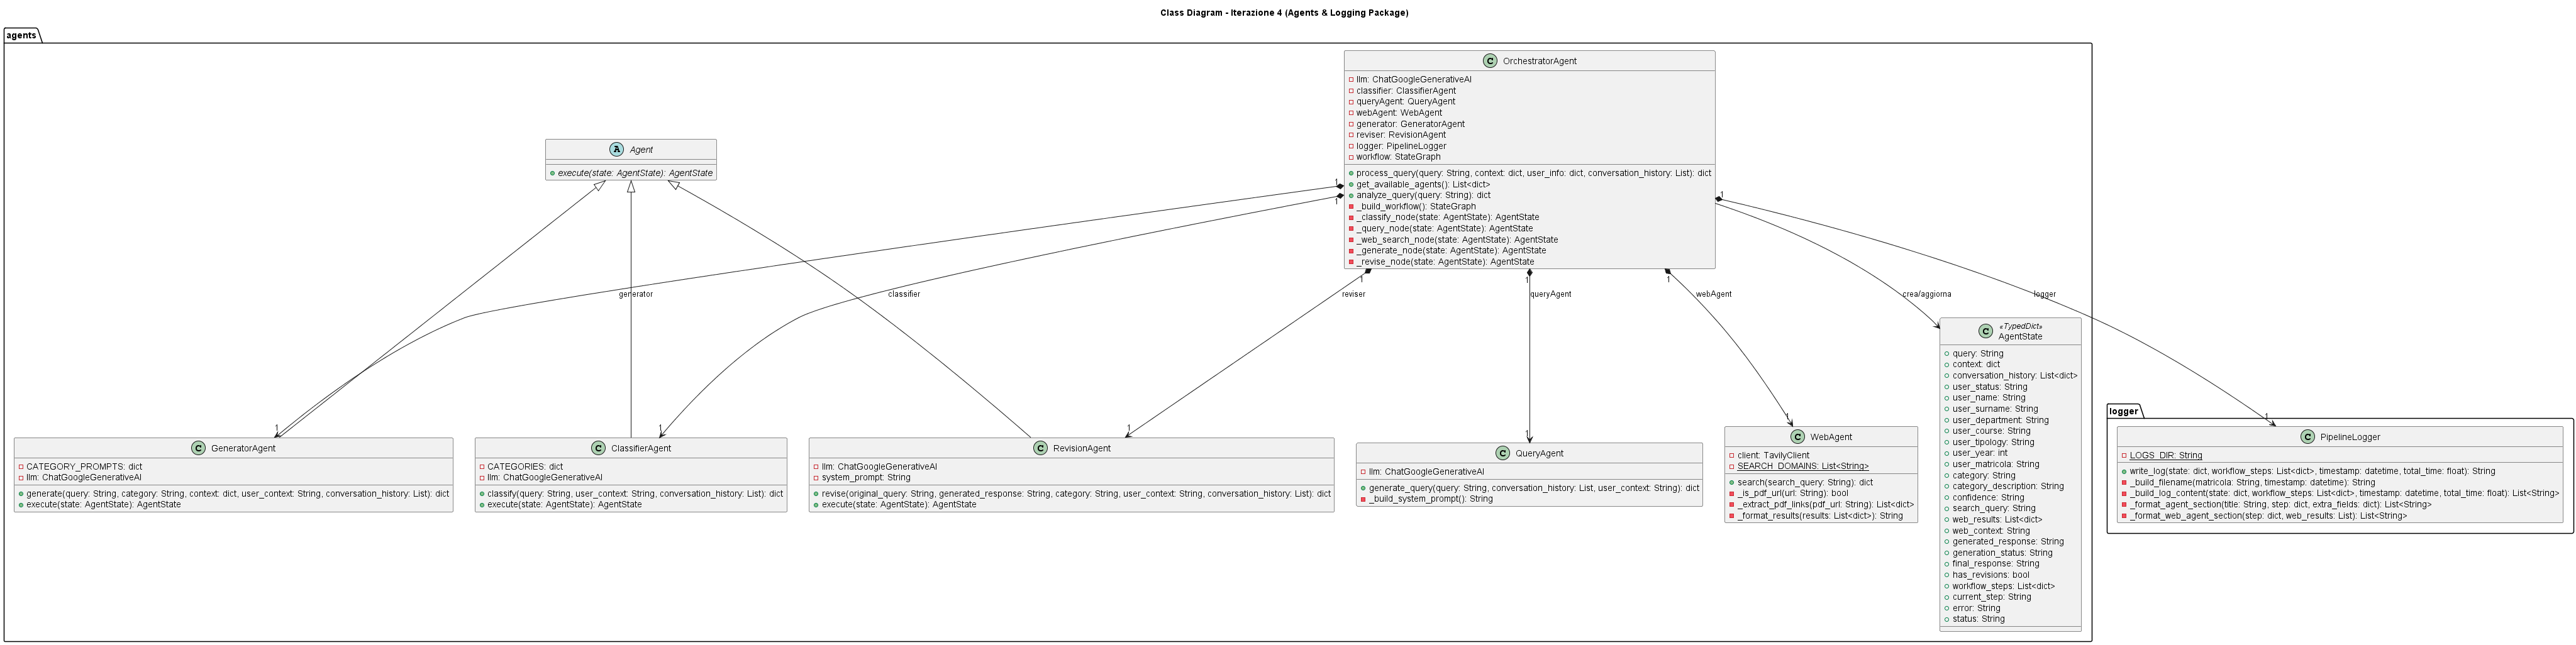
\includegraphics[width=\textwidth]{class_agents_diagram4}
\caption{Diagramma delle classi -- Agenti (Iterazione 4)}
\end{figure}

\begin{figure}[H]
\centering
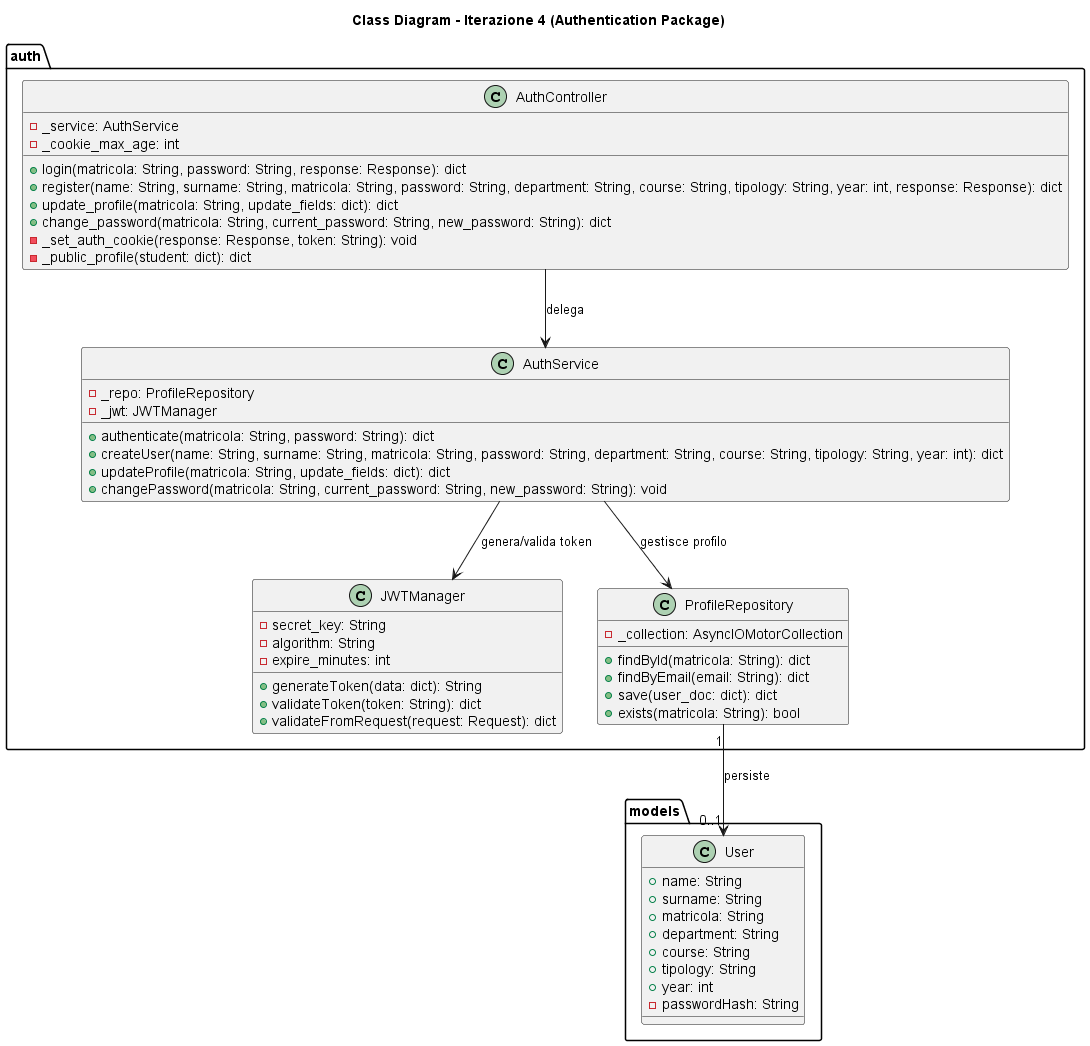
\includegraphics[width=0.9\textwidth]{class_auth_diagram4}
\caption{Diagramma delle classi -- Layer Auth (Iterazione 4)}
\end{figure}

\begin{figure}[H]
\centering
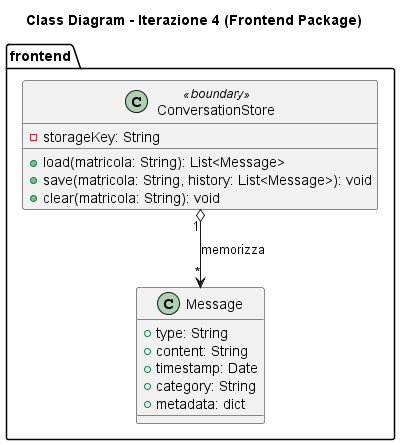
\includegraphics[width=0.8\textwidth]{class_frontend_diagram4}
\caption{Diagramma delle classi -- Frontend React (Iterazione 4)}
\end{figure}

\subsection{Diagramma di Sequenza}

\begin{figure}[H]
\centering
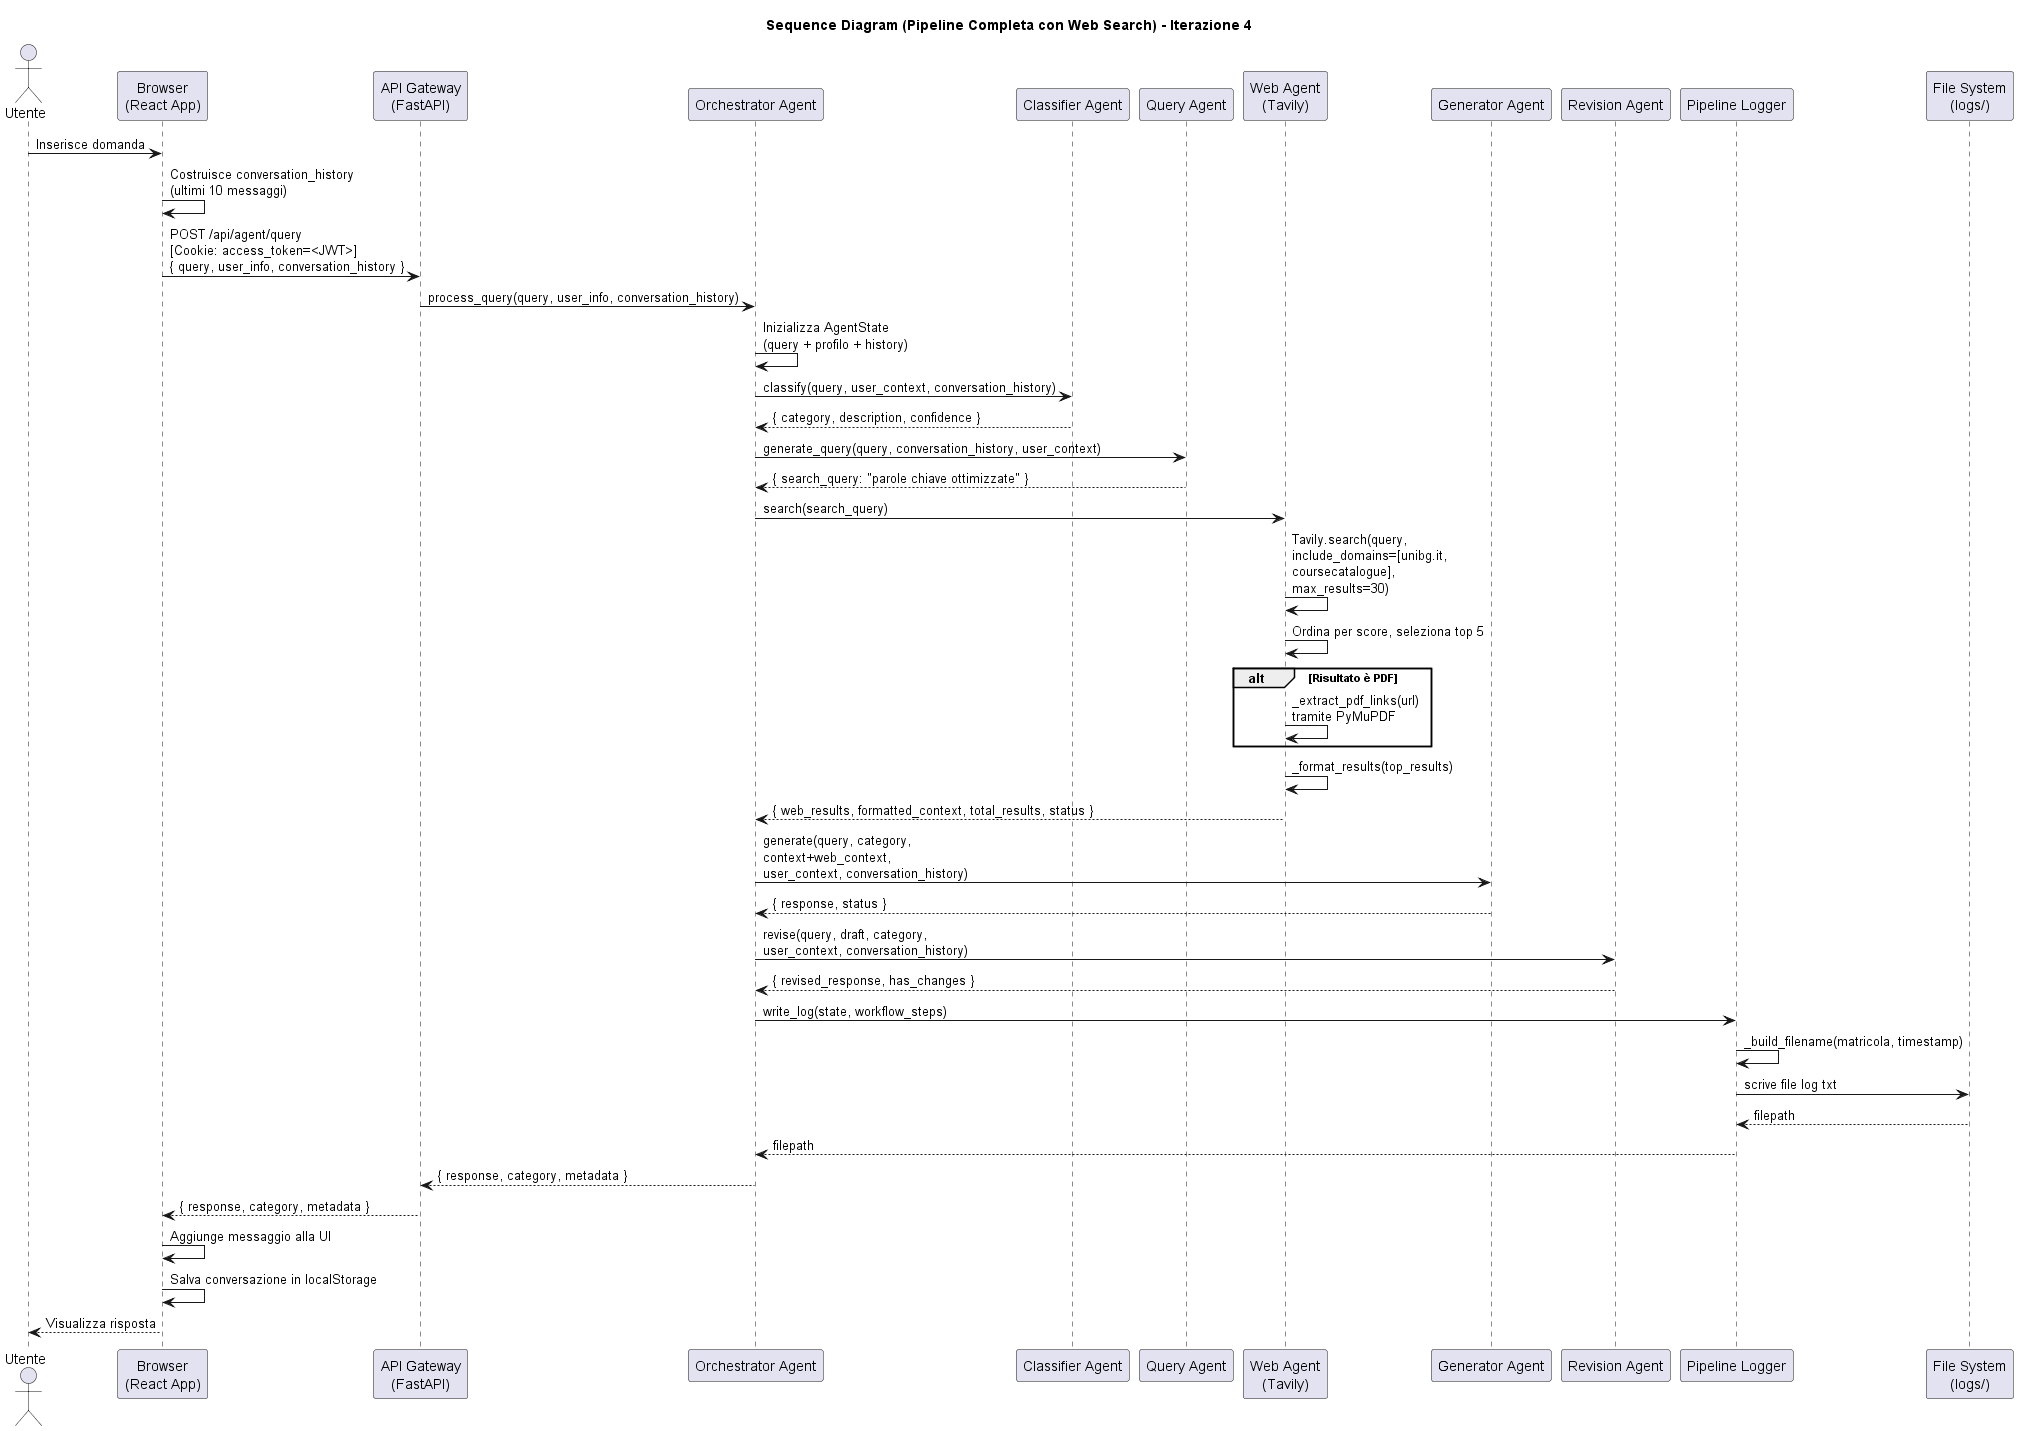
\includegraphics[width=\textwidth]{sequence_diagram4}
\caption{Diagramma di sequenza -- Pipeline completa con web search/exam extract (Iterazione 4)}
\end{figure}

\subsection{Diagramma di Attività}

\begin{figure}[H]
\centering
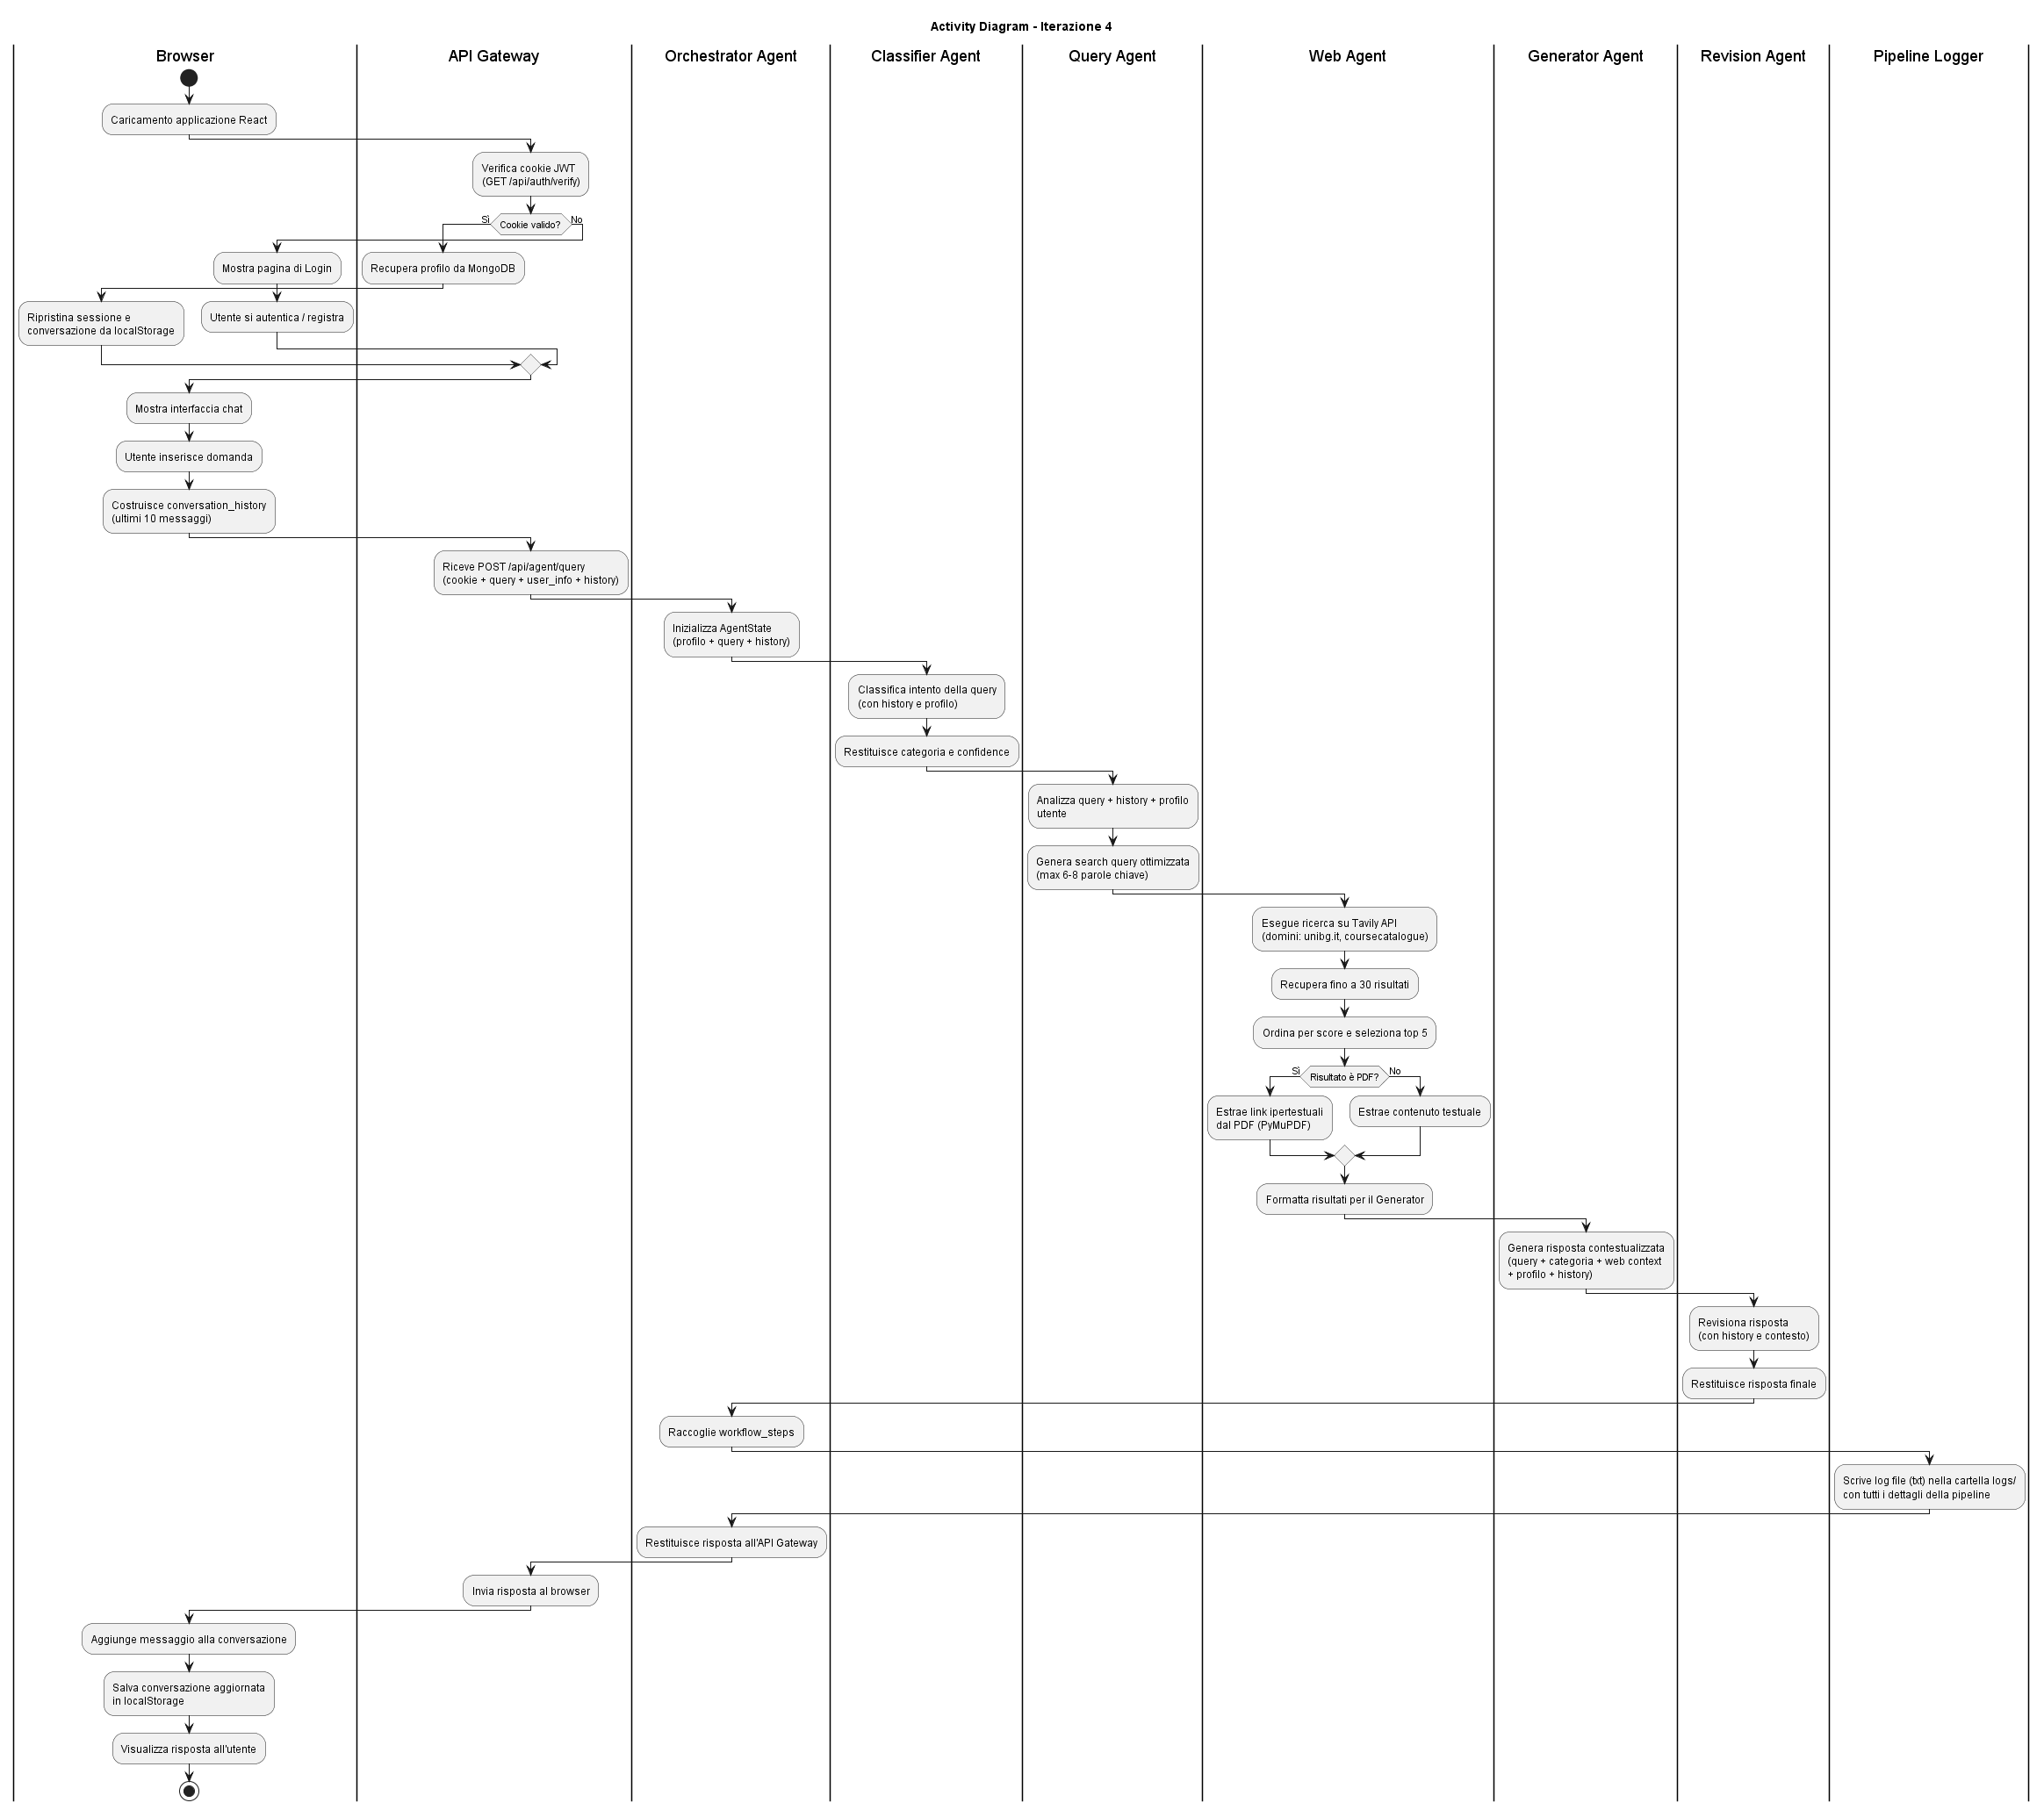
\includegraphics[width=0.75\textwidth]{activity_diagram4}
\caption{Diagramma di attività -- Flusso con routing condizionale (Iterazione 4)}
\end{figure}

\subsection{Algoritmi e Complessità}

\paragraph{Web Search Standard.}
Tavily search ($O(T)$, I/O rete) $\rightarrow$ sort $N \leq 30$ risultati ($O(N \log N) = O(1)$) $\rightarrow$ top 5 $\rightarrow$ estrazione PDF ($O(P)$ pagine). Totale: $O(T + P)$.

\paragraph{Exam Extract.}
Recupero calendari $O(1)$ (dizionario statico) $\rightarrow$ costruzione opzioni $O(K)$ $\rightarrow$ LLM sceglie calendario $O(L)$ $\rightarrow$ Tavily Extract $O(T)$ $\rightarrow$ web search supplementare $O(T)$. Totale: $O(L + 2T)$, circa il doppio di una ricerca standard.

\paragraph{Pipeline Logger.}
Costruzione log $O(S \cdot R)$ dove $S=5$ step e $R$ è la dimensione dei contenuti. Scrittura su disco $O(R)$. Non bloccante.

\paragraph{Cambio LLM Provider.}

\begin{table}[H]
\centering
\begin{tabularx}{\textwidth}{l X X}
\toprule
\textbf{Aspetto} & \textbf{Groq / LLaMA 3.3 70B} & \textbf{Google Gemini 2.5 Flash} \\
\midrule
Context window & 128K token & 1M token \\
Qualità ragionamento & Alta & Molto alta \\
Gestione contesti lunghi & Limitata & Ottima \\
\bottomrule
\end{tabularx}
\caption{Confronto LLM provider}
\end{table}

\section{Testing Dinamico}

\begin{table}[H]
\centering
\small
\begin{tabularx}{\textwidth}{l l l X l}
\toprule
\textbf{ID} & \textbf{Endpoint} & \textbf{Met.} & \textbf{Descrizione} & \textbf{Atteso} \\
\midrule
IT4-01 & \texttt{/api/agent/query} & POST & Query con web search & 200 \\
IT4-02 & \texttt{/api/agent/query} & POST & Query date esami & 200 \\
IT4-03 & \texttt{/api/agent/query} & POST & Verifica ottimizzazione query & 200 \\
IT4-04 & \texttt{/api/agent/analyze} & POST & Analisi debug & 200 \\
IT4-05 & \texttt{/api/agent/query} & POST & Follow-up date esami & 200 \\
\bottomrule
\end{tabularx}
\caption{Test API -- Iterazione 4 (5 test, 2 endpoint)}
\end{table}

\textbf{Asserzioni chiave}:
\begin{itemize}
    \item La pipeline contiene 5 step: classification, query\_generation, web\_search (o exam\_extract), generation, revision
    \item Ogni step ha \texttt{elapsed\_time} per il monitoraggio delle performance
    \item Il QueryAgent produce query ottimizzate ($<$ 100 caratteri)
    \item Il branching \texttt{date\_esami} $\rightarrow$ \texttt{exam\_extract} funziona correttamente
\end{itemize}

\textbf{Esecuzione automatizzata}:
\begin{verbatim}
newman run postman_collection.json --folder "Iterazione 4"
\end{verbatim}

\section{Analisi Statica del Codice}
\label{sec:analisi-statica-completa}

L'analisi statica completa è stata condotta con \textbf{radon} sull'intero codebase dell'Iterazione 4.

\subsection{Complessità Ciclomatica (McCabe)}

\begin{table}[H]
\centering
\small
\begin{tabularx}{\textwidth}{l l X l}
\toprule
\textbf{File} & \textbf{Grado Max} & \textbf{Funzione Più Complessa} & \textbf{CC} \\
\midrule
\texttt{orchestrator\_agent.py} & A & \texttt{\_generate\_node} & 4 \\
\texttt{classifier\_agent.py} & B & \texttt{classify} & 6 \\
\texttt{generator\_agent.py} & B & \texttt{generate} & 6 \\
\texttt{query\_agent.py} & B & \texttt{generate\_query} & 6 \\
\texttt{revision\_agent.py} & B & \texttt{revise} & 6 \\
\texttt{web\_agent.py} & \textbf{C} & \texttt{\_select\_calendar\_link} & \textbf{11} \\
\texttt{agent\_state.py} & A & \texttt{build\_user\_context} & 2 \\
\texttt{auth/controller.py} & A & Tutte & 1 \\
\texttt{auth/service.py} & A & \texttt{authenticate} & 3 \\
\texttt{auth/jwt\_manager.py} & A & \texttt{\_\_init\_\_} & 2 \\
\texttt{auth/profile\_repository.py} & A & \texttt{updateProfile} & 4 \\
\texttt{pipeline\_logger.py} & B & \texttt{\_build\_log\_content} & 8 \\
\texttt{models/user.py} & A & Tutte & 1 \\
\texttt{main.py} & A & \texttt{verify\_auth} & 3 \\
\texttt{config.py} & A & \texttt{Settings} & 1 \\
\bottomrule
\end{tabularx}
\caption{Complessità ciclomatica per file}
\end{table}

\textbf{Distribuzione}: 90.3\% grado A (93 blocchi), 8.7\% grado B (9 blocchi), 1.0\% grado C (1 blocco). Nessun blocco D o F. \textbf{Media: A (2.37)}.

\textbf{Punto critico}: \texttt{WebAgent.\_select\_calendar\_link} (CC=11, grado C) è la funzione più complessa. La complessità è dovuta alla costruzione dinamica delle opzioni, all'invocazione LLM e al parsing multi-pattern con fallback.

\subsection{Indice di Manutenibilità}

\begin{table}[H]
\centering
\small
\begin{tabularx}{\textwidth}{l l l l}
\toprule
\textbf{File} & \textbf{MI} & \textbf{Grado} & \textbf{Valutazione} \\
\midrule
\texttt{auth/controller.py} & 100.00 & A & Eccellente \\
\texttt{models/user.py} & 100.00 & A & Eccellente \\
\texttt{config.py}, \texttt{db.py} & 100.00 & A & Eccellente \\
\texttt{auth/jwt\_manager.py} & 86.28 & A & Molto buono \\
\texttt{agent\_state.py} & 84.86 & A & Molto buono \\
\texttt{auth/profile\_repository.py} & 81.33 & A & Molto buono \\
\texttt{auth/service.py} & 80.09 & A & Molto buono \\
\texttt{query\_agent.py} & 75.73 & A & Buono \\
\texttt{classifier\_agent.py} & 73.03 & A & Buono \\
\texttt{generator\_agent.py} & 72.44 & A & Buono \\
\texttt{revision\_agent.py} & 71.59 & A & Buono \\
\texttt{main.py} & 64.17 & A & Accettabile \\
\texttt{orchestrator\_agent.py} & 56.60 & A & Accettabile \\
\texttt{web\_agent.py} & 52.21 & A & Accettabile \\
\texttt{pipeline\_logger.py} & 51.85 & A & Accettabile \\
\bottomrule
\end{tabularx}
\caption{Indice di manutenibilità per file}
\end{table}

\textbf{Tutti i file hanno grado A} (MI $>$ 20). Il layer Auth conferma MI eccellente (80--100).

\subsection{Metriche Raw (LOC)}

\begin{table}[H]
\centering
\begin{tabularx}{\textwidth}{l r r r r}
\toprule
\textbf{Modulo} & \textbf{LOC} & \textbf{SLOC} & \textbf{Commenti} & \textbf{\%} \\
\midrule
\texttt{agents/} (7 file) & 1408 & 1000 & 83 & 58.1\% \\
\texttt{logger/} (2 file) & 350 & 243 & 22 & 14.4\% \\
\texttt{auth/} (5 file) & 327 & 194 & 4 & 13.5\% \\
\texttt{main.py} & 224 & 153 & 5 & 9.2\% \\
\texttt{models/} (2 file) & 69 & 43 & 0 & 2.8\% \\
\texttt{config.py} + \texttt{db.py} & 45 & 22 & 6 & 1.9\% \\
\midrule
\textbf{Totale} & \textbf{2423} & \textbf{1655} & \textbf{120} & \textbf{100\%} \\
\bottomrule
\end{tabularx}
\caption{Distribuzione LOC per modulo}
\end{table}

\subsection{Riepilogo e Raccomandazioni}

\textbf{Punti di forza}:
\begin{itemize}
    \item Complessità bassa: media CC = 2.37 (grado A), solo 1/103 funzioni in grado C
    \item Alta manutenibilità: tutti i file MI $>$ 20 (grado A)
    \item Design pulito layer Auth: CC $\leq$ 3
    \item Codebase compatto: 2423 LOC totali
\end{itemize}

\textbf{Aree di miglioramento}:
\begin{itemize}
    \item \texttt{web\_agent.py}: estrarre il parsing della risposta LLM in un metodo dedicato (CC=11 $\rightarrow$ 2$\times$CC=5)
    \item \texttt{orchestrator\_agent.py}: 437 LOC, valutare estrazione nodi in file separati
    \item \texttt{LoginPage.jsx} / \texttt{SettingsPage.jsx}: \texttt{DIPARTIMENTI\_CORSI} duplicato, estrarre in \texttt{constants.js}
\end{itemize}


% ═══════════════════════════════════════════════════════════════════
% CHAPTER 7 – ITERAZIONE 5 (WIP)
% ═══════════════════════════════════════════════════════════════════
\chapter{Iterazione 5 -- Gestione Profilo Utente e Miglioramenti (WIP)}

\section{Obiettivo dell'Iterazione}

L'Iterazione 5, attualmente \textit{work in progress}, si concentra su:
\begin{itemize}
    \item \textbf{Gestione profilo utente dal frontend}: modifica dati personali e cambio password
    \item \textbf{Miglioramento del ClassifierAgent}: categorizzazione più precisa
\end{itemize}

\section{Analisi dei Requisiti e Use Case}

\subsection{Use Case}

\begin{itemize}
    \item \textbf{UC-14 -- Modifica Profilo Utente}: \texttt{PUT /api/auth/profile} con body opzionale. JWT richiesto. I campi \texttt{passwordHash}, \texttt{matricola}, \texttt{\_id} sono esclusi per sicurezza.

    \item \textbf{UC-15 -- Cambio Password}: \texttt{PUT /api/auth/password} con \texttt{current\_password} e \texttt{new\_password}. Verifica password corrente prima dell'aggiornamento.
\end{itemize}

\subsection{Endpoint API -- Nuovi}

\begin{table}[H]
\centering
\begin{tabularx}{\textwidth}{l l X}
\toprule
\textbf{Metodo} & \textbf{Path} & \textbf{Descrizione} \\
\midrule
PUT & \texttt{/api/auth/profile} & Aggiorna i dati del profilo utente \\
PUT & \texttt{/api/auth/password} & Cambia la password dell'utente \\
\bottomrule
\end{tabularx}
\caption{Nuovi endpoint API -- Iterazione 5}
\end{table}

\subsection{Funzionalità Implementate (Parziale)}

\textbf{Backend}:
\begin{itemize}
    \item Modelli Pydantic: \texttt{UpdateProfileRequest} (campi opzionali), \texttt{ChangePasswordRequest}
    \item \texttt{ProfileRepository}: \texttt{updateProfile()}, \texttt{updatePassword()}
    \item \texttt{AuthService}: \texttt{updateProfile()}, \texttt{changePassword()}
    \item \texttt{AuthController}: \texttt{update\_profile()}, \texttt{change\_password()}
\end{itemize}

\textbf{Frontend}:
\begin{itemize}
    \item \texttt{SettingsPage.jsx}: form di modifica profilo e cambio password, accessibile via icona ingranaggio (solo utenti autenticati)
    \item Aggiornamento stato React dopo modifica riuscita
\end{itemize}

\subsection{Miglioramento ClassifierAgent}

\begin{itemize}
    \item Affinamento prompt per ridurre ambiguità
    \item Migliore gestione domande follow-up con cambio contesto
    \item Possibile introduzione di sotto-categorie per \texttt{generale}
\end{itemize}

\section{Design dell'Architettura}

In fase di definizione. L'architettura resta quella dell'Iterazione 4 con aggiunta dei nuovi endpoint e componente \texttt{SettingsPage}.

\section{Testing Dinamico}

In corso. I test IT2-08 (aggiornamento profilo) e IT2-09/IT2-10 (cambio password) coprono già i nuovi endpoint.

\section{Analisi Statica del Codice}

In corso; i nuovi metodi nel layer Auth mantengono complessità A (CC $\leq$ 4) in linea con il pattern esistente.


% ═══════════════════════════════════════════════════════════════════
% CHAPTER 8 – SCELTE ARCHITETTURALI E DI PROGETTO
% ═══════════════════════════════════════════════════════════════════
\chapter{Scelte Architetturali e di Progetto}

\section{Architettura Multi-Agent con LangGraph}

La scelta fondamentale è l'adozione di un'architettura \textbf{multi-agent} orchestrata tramite LangGraph:

\begin{table}[H]
\centering
\begin{tabularx}{\textwidth}{l X}
\toprule
\textbf{Agente} & \textbf{Responsabilità} \\
\midrule
ClassifierAgent & Classificazione dell'intento in 7 categorie \\
QueryAgent & Generazione di query di ricerca web ottimizzate \\
WebAgent & Ricerca web su Tavily + estrazione calendari esami \\
GeneratorAgent & Generazione risposta con prompt per categoria \\
RevisionAgent & Revisione per correttezza, struttura, concisione \\
OrchestratorAgent & Coordinamento workflow completo \\
\bottomrule
\end{tabularx}
\caption{Responsabilità degli agenti}
\end{table}

\textbf{Motivazione}: la separazione permette di modificare/sostituire un agente senza impattare gli altri, aggiungere nodi, testare in isolamento e implementare routing condizionale.

\section{Pattern AgentState (Shared State)}

Lo stato della pipeline è gestito tramite \texttt{TypedDict} condiviso tra i nodi del grafo. Garantisce: tracciabilità (\texttt{workflow\_steps}), fallback robusti e estensibilità (nuovi campi senza modifiche ai nodi esistenti).

\section{Scelta del LLM Provider}

\begin{enumerate}
    \item \textbf{Iterazioni 1--3}: Groq / LLaMA 3.3 70B (bassa latenza, buona qualità)
    \item \textbf{Iterazione 4+}: Google Gemini 2.5 Flash (context 1M token, ragionamento superiore)
\end{enumerate}

Il cambio è \textbf{trasparente}: l'LLM è iniettato dall'OrchestratorAgent, nessun agente ha riferimenti hardcoded.

\section{Autenticazione con httpOnly Cookie}

Motivazione:
\begin{itemize}
    \item \textbf{Protezione XSS}: token inaccessibile da JavaScript
    \item \textbf{Semplicità}: il browser allega automaticamente il cookie
    \item \textbf{SameSite=lax}: protezione CSRF di base
\end{itemize}

\section{Memoria Conversazionale lato Client}

localStorage scelto per semplicità, nessun overhead infrastrutturale, adeguatezza per il caso d'uso (singolo browser). Limitazione a 10 messaggi per contenere il context window.

\section{Tavily API per la Ricerca Web}

Scelto per: filtering per dominio, \texttt{search\_depth="advanced"}, funzionalità \texttt{extract()}, restituzione \texttt{raw\_content}.

\section{Routing Condizionale per Date Esami}

Motivato dalla specificità: calendari organizzati per polo/sessione con URL specifiche; ricerca generica insufficiente; Tavily Extract per contenuto completo; selezione LLM del calendario corretto.

\section{Sicurezza}

\begin{itemize}
    \item Password hashate con bcrypt (salt incluso), mai in chiaro
    \item JWT HMAC-SHA256, scadenza 7 giorni, httpOnly cookie
    \item CORS origini esplicite, \texttt{allow\_credentials=True}
    \item \texttt{passwordHash} filtrato da ogni risposta API
    \item Update profile: \texttt{passwordHash}, \texttt{matricola}, \texttt{\_id} esclusi
\end{itemize}

\section{Containerizzazione}

Docker Compose: backend Python isolato, frontend Nginx con build Vite, MongoDB Atlas esterno (SaaS), volumi per hot-reload.


% ═══════════════════════════════════════════════════════════════════
% CHAPTER 9 – CONCLUSIONI
% ═══════════════════════════════════════════════════════════════════
\chapter{Conclusioni e Sviluppi Futuri}

\section{Riepilogo delle Iterazioni}

\begin{table}[H]
\centering
\small
\begin{tabularx}{\textwidth}{l X}
\toprule
\textbf{Iterazione} & \textbf{Funzionalità Principali} \\
\midrule
0 -- Visione & Requisiti, user stories, architettura target \\
1 -- MVP & Pipeline classify $\rightarrow$ generate $\rightarrow$ revise (Groq/LLaMA) \\
2 -- Auth & Registrazione, login, MongoDB, personalizzazione, React, Docker \\
3 -- Sessione & JWT httpOnly cookie, verify/logout, localStorage memory, auth refactoring \\
4 -- Web \& Esami & QueryAgent, WebAgent (Tavily), date\_esami con routing condizionale, PipelineLogger, Gemini 2.5 Flash \\
5 -- Profilo (WIP) & Modifica profilo utente, cambio password, miglioramenti classifier \\
\bottomrule
\end{tabularx}
\caption{Riepilogo iterazioni}
\end{table}

\section{Riepilogo dei Test}

\begin{table}[H]
\centering
\begin{tabularx}{\textwidth}{l r r X}
\toprule
\textbf{Iterazione} & \textbf{N. Test} & \textbf{Endpoint} & \textbf{Copertura} \\
\midrule
IT1 & 6 & 4 & Pipeline base, health check, lista agenti \\
IT2 & 12 & 7 & Auth completa (register, login, verify, profile, password, logout) \\
IT3 & 5 & 2 & Memoria conversazionale, follow-up, cronologia \\
IT4 & 5 & 2 & Pipeline completa, exam extract, debug \\
\midrule
\textbf{Totale} & \textbf{28} & \textbf{10} & Tutti gli endpoint REST \\
\bottomrule
\end{tabularx}
\caption{Riepilogo dei test per iterazione}
\end{table}

\section{Obiettivi Raggiunti}

\begin{itemize}
    \item Pipeline multi-agent con 5 agenti specializzati
    \item Classificazione automatica in 7 categorie
    \item Recupero informazioni reali da \texttt{unibg.it} tramite Tavily
    \item Flusso dedicato date esami con selezione intelligente calendario
    \item Autenticazione JWT httpOnly cookie
    \item Personalizzazione risposte basata sul profilo
    \item Memoria conversazionale per coerenza contestuale
    \item Logging completo per diagnostica
    \item Deploy containerizzato Docker Compose
    \item Codebase con complessità media A (CC=2.37) e manutenibilità A su tutti i file
\end{itemize}

\section{Sviluppi Futuri}

\begin{itemize}
    \item Completamento Iterazione 5 (profilo utente, classifier)
    \item Refresh token per rinnovo JWT
    \item Persistenza conversazione su backend (MongoDB)
    \item Re-ranking semantico risultati web
    \item Log consultabili via API REST
    \item Deploy HTTPS con \texttt{secure=True} sul cookie
    \item Aggiornamento automatico calendari esami
\end{itemize}

\section{Considerazioni sulla Metodologia AMDD}

L'approccio AMDD si è rivelato efficace:
\begin{itemize}
    \item La visione iniziale (Iterazione 0) ha fornito direzione senza vincolare le scelte implementative
    \item Ogni iterazione ha prodotto un incremento funzionante e testabile
    \item I modelli UML sono stati creati ``just enough'' per documentare le scelte
    \item Le decisioni architetturali (cambio LLM, routing condizionale) sono emerse naturalmente
    \item L'approccio incrementale ha permesso di scoprire e risolvere problemi senza rework massivo
\end{itemize}

\end{document}
